\documentclass[conference]{IEEEtran}
\IEEEoverridecommandlockouts

\usepackage{cite}
\usepackage{amsmath,amssymb,amsfonts}
\usepackage{algorithmic}
\usepackage{graphicx}
\usepackage{textcomp}
\usepackage{xcolor}
\usepackage{colortbl}
\usepackage{booktabs}
\usepackage{tabularx}
\usepackage{multirow}
\usepackage{url}
\usepackage{microtype}
\usepackage{balance}
\usepackage{stfloats}
\usepackage{tcolorbox}
\tcbuselibrary{skins}

% Visual Styling Palette: IEEE Prestige
\definecolor{ieeeblue}{RGB}{0, 45, 114}
\definecolor{slateheader}{RGB}{30, 41, 59}
\definecolor{subheadergray}{RGB}{71, 85, 105}
\definecolor{tableheader}{RGB}{236, 242, 250}
\definecolor{tablerowalt}{RGB}{248, 250, 252}
\definecolor{highlightgreen}{RGB}{236, 253, 243}
\definecolor{highlightpink}{RGB}{254, 242, 242}
\definecolor{critred}{RGB}{185, 28, 28}
\definecolor{slackblue}{RGB}{29, 78, 216}
\definecolor{cardbg}{RGB}{250, 252, 255}
\definecolor{cardborder}{RGB}{195, 212, 233}

% Distinct Section Heading Architecture
\makeatletter
\def\section{\@startsection{section}{1}{\z@}{2.4ex plus 1.0ex minus 0.5ex}%
{1.0ex plus 0.4ex minus 0.2ex}{\normalfont\large\bfseries\color{ieeeblue}}}
\def\subsection{\@startsection{subsection}{2}{\z@}{1.8ex plus 0.8ex minus 0.4ex}%
{0.8ex plus 0.3ex minus 0.2ex}{\normalfont\normalsize\bfseries\color{slateheader}}}
\def\subsubsection{\@startsection{subsubsection}{3}{\z@}{1.3ex plus 0.6ex minus 0.3ex}%
{0.5ex plus 0.2ex minus 0.1ex}{\normalfont\normalsize\bfseries\itshape\color{subheadergray}}}
\makeatother

% Spacing & Layout Optimization
\setlength{\textfloatsep}{8pt plus 2pt minus 2pt}
\setlength{\floatsep}{6pt plus 2pt minus 2pt}
\setlength{\intextsep}{6pt plus 2pt minus 2pt}
\setlength{\dbltextfloatsep}{8pt plus 2pt minus 2pt}
\setlength{\dblfloatsep}{6pt plus 2pt minus 2pt}

\renewcommand{\topfraction}{0.95}
\renewcommand{\bottomfraction}{0.95}
\renewcommand{\textfraction}{0.05}
\renewcommand{\floatpagefraction}{0.85}
\renewcommand{\dbltopfraction}{0.95}
\renewcommand{\dblfloatpagefraction}{0.85}

% Architectural Diagram Card Environment
\newtcolorbox{diagramcard}[2][]{%
  colback=cardbg,
  colframe=cardborder,
  coltitle=ieeeblue,
  fonttitle=\bfseries\sffamily\footnotesize,
  title={#2},
  boxrule=0.75pt,
  arc=3pt,
  left=5pt,right=5pt,top=5pt,bottom=5pt,
  before upper={\centering},
  #1
}

% Graphics directory
\graphicspath{{../docs/figures/}}

\begin{document}

\title{\LARGE\bfseries AP-CWS: Predictive Cold-Start-Aware Serverless Workflow Scheduler}

\author{
\IEEEauthorblockN{Nikhil Sharma\IEEEauthorrefmark{1}, Raghav Arora\IEEEauthorrefmark{1}, and Jashanpreet Singh\IEEEauthorrefmark{1}}
\IEEEauthorblockA{\IEEEauthorrefmark{1}Department of Mechanical Engineering, Indian Institute of Technology (BHU) Varanasi, India}
}

\maketitle

\begin{abstract}
Serverless computing platforms execute complex event-driven applications as Directed Acyclic Graphs (DAGs). In these workflows, cascading cold starts along the critical execution path severely degrade performance. When an uninstantiated function initializes on a critical path, downstream tasks stall, inflating tail latency and causing Service-Level Objective (SLO) violations. Existing schedulers decouple warm pool sizing from DAG topology, allocating containers based on aggregate invocation frequency. This strategy wastes physical memory on non-critical tasks while leaving critical tasks vulnerable to initialization delays. This paper presents AP-CWS, a predictive workflow scheduler that coordinates warm container pool sizing and task placement. AP-CWS combines Holt linear exponential smoothing, DAG topological slack budgeting, joint placement scoring, and Just-In-Time (JIT) successor prewarming. To support high-throughput clusters, we introduce Fast-AP-CWS, which uses memoized DAG metrics and power-of-two-choices node selection to achieve $O(1)$ dispatch time. We evaluated the scheduler across 324 discrete-event simulation runs using three representative workflow topologies under four empirical arrival patterns. Across these evaluations, AP-CWS achieves an overall P95 tail latency of 2.83~s, representing a 27.8\% reduction compared to state-of-the-art baselines. Critical-path cold starts drop to 0.63\%, and contractual SLO violations decrease by 84.4\% alongside a 4.6\% reduction in total execution cost.
\end{abstract}

\begin{IEEEkeywords}
Serverless computing, Function-as-a-Service (FaaS), Directed Acyclic Graph (DAG), cold start, tail latency, critical path, workflow scheduling, resource allocation, discrete-event simulation.
\end{IEEEkeywords}

\begin{table*}[t]
\centering
\caption{System Notation, Mathematical Symbols, and Operational Definitions}
\label{tab:notation}
\footnotesize
\setlength{\tabcolsep}{5pt}
\renewcommand{\arraystretch}{1.12}
\resizebox{\textwidth}{!}{%
\begin{tabular}{llll}
\toprule
\rowcolor{tableheader}
\textbf{Symbol / Variable} & \textbf{Structural Category} & \textbf{Operational Definition \& Mechanistic Role} & \textbf{Physical Dimension / Domain} \\
\midrule
$\mathcal{G} = (\mathcal{V}, \mathcal{E})$ & Workflow Model & Directed Acyclic Graph of constituent function tasks $\mathcal{V}$ and precedence dependency edges $\mathcal{E}$ & Topological graph structure \\
\rowcolor{tablerowalt}
$f_i \in \mathcal{V}$ & Workflow Task & Individual serverless function task instance ($i \in \{1, \dots, N\}$) & Discrete execution entity \\
$e_{ik} = (f_i, f_k)$ & Dependency Edge & Precedence constraint requiring complete termination of parent $f_i$ before dispatching child $f_k$ & Precedence pair in $\mathcal{V} \times \mathcal{V}$ \\
\rowcolor{tablerowalt}
$m_i, c_i$ & Task Resource & DRAM memory allocation requirement and normalized CPU core quota demanded by function $f_i$ & Megabytes (MB), Cores \\
$t_i^{base} \ (\bar{t}_i), s_i$ & Execution Profile & Nominal computational execution duration on baseline node ($v=1.0$) and container startup cold delay & Seconds (s) \\
\rowcolor{tablerowalt}
$d_{ik}$ & State Transfer & Intermediate serialized application state data transferred across dependency edge $(f_i, f_k)$ & Megabytes (MB) \\
$EST_i, EFT_i$ & Topological Timing & Earliest Start Time and Earliest Finish Time computed via forward topological traversal of $\mathcal{G}$ & Seconds (s) \\
\rowcolor{tablerowalt}
$LFT_i, LST_i$ & Topological Timing & Latest Finish Time and Latest Start Time computed via backward topological traversal from sink nodes & Seconds (s) \\
$T^*$ & Critical Makespan & Theoretical minimum workflow completion time along the zero-slack critical execution path & Seconds (s) \\
\rowcolor{tablerowalt}
$\text{Slack}_i$ & Execution Slack & Spare delay buffer before downstream delay propagation ($\text{Slack}_i = LST_i - EST_i$) & Seconds (s) \\
$K_i$ & Criticality Index & Dimensionless topological urgency index: $K_i = 1 - (\text{Slack}_i / T^*)$; sensitivity to startup delay & Real interval $[0, 1]$ \\
\rowcolor{tablerowalt}
$\mathcal{J}$ & Compute Cluster & Heterogeneous worker nodes available for container placement and execution ($j \in \{1, \dots, M\}$) & Node set \\
$M_j, C_j$ & Physical Capacity & Total physical DRAM memory and total hardware processing cores available on worker node $j$ & MB, Physical Cores \\
\rowcolor{tablerowalt}
$v_j, p_j$ & Node Specifications & Hardware CPU speed scaling multiplier ($t_{ij} = t_i^{base} / v_j$) and active unit financial billing tariff & Multiplier, \$/GB-hr \\
$\tau_{ik}^{net}(j, j')$ & Network Latency & Inter-node data serialization and transmission delay ($0$ if co-located; $d_{ik}/B_{net} + \delta_{prop}$ if cross-node) & Seconds (s) \\
\rowcolor{tablerowalt}
$\Delta$ & Planning Interval & Periodic offline control loop epoch for Holt demand forecasting and warm pool dimensioning & Seconds ($\Delta = 60\text{ s}$) \\
$L_t, T_t$ & Demand State & Smoothed base level and trend slope components updated via Holt linear exponential smoothing & Invocations/s \\
\rowcolor{tablerowalt}
$\alpha, \beta$ & Smoothing Weights & Moving level weight and trend updating coefficients ($\alpha = 0.20, \beta = 0.10$) & Real interval $[0, 1]$ \\
$\hat{\lambda}_i$ & Projected Demand & Forecasted invocation arrival rate for function $f_i$ across subsequent planning window $\Delta$ & Invocations/s \\
\rowcolor{tablerowalt}
$p_i^{target}$ & Reliability Budget & Target allowable cold-start probability ceiling assigned to task $f_i$ based on criticality $K_i$ & Real interval $[0, 1]$ \\
$W_i^*, W_{ij}$ & Warm Pool Sizing & Target cluster-wide warm container quota and discrete warm container pool allocated on node $j$ & Non-negative integers $\mathbb{Z}_{\ge 0}$ \\
\rowcolor{tablerowalt}
$x_{ij} \in \{0, 1\}$ & Placement Indicator & Binary decision variable: $1$ if task instance $f_i$ is dispatched to worker node $j$, and $0$ otherwise & Boolean binary \\
$y_{ij} \in \{0, 1\}$ & Startup Status & Binary state flag: $0$ if warm container is acquired on node $j$, and $1$ if cold initialization is incurred & Boolean binary \\
\rowcolor{tablerowalt}
$S_{ij}$ & Dispatch Objective & Multi-factor cost-latency placement evaluation score quantifying suitability of node $j$ for task $f_i$ & Scalar value \\
$\mu, \gamma$ & Tuning Weights & Relative financial cost penalty weight ($\mu = 0.05$) and unreserved memory headroom bonus ($\gamma = 0.10$) & Scalar coefficients \\
\rowcolor{tablerowalt}
$\kappa$ & Prewarm Threshold & Criticality threshold triggering asynchronous Just-In-Time (JIT) successor container prewarming & Criticality threshold ($\kappa = 0.60$) \\
$d$ & Sub-Sampling Size & Number of randomly sampled candidate nodes evaluated under Power-of-Two-Choices in Fast-AP-CWS & Integer ($d = 2 \ll |\mathcal{J}|$) \\
\rowcolor{tablerowalt}
$T_{P95}, T_{SLO}$ & Quality Metric & Measured 95th-percentile end-to-end workflow completion time and target contractual deadline & Seconds (s) \\
\bottomrule
\end{tabular}%
}
\end{table*}

\section{Introduction}
\label{sec:intro}
Serverless computing, commonly formalized as Function-as-a-Service (FaaS), has become the prevailing execution paradigm for modern event-driven cloud applications~\cite{shahrad2020serverless, openwhisk2023}. Developers structure application logic as granular, stateless functions while cloud providers automate infrastructure provisioning, auto-scaling, and fault tolerance. Platforms bill users strictly for active execution time in sub-second increments. This elastic execution model suits bursty, event-driven applications.

Modern cloud architectures increasingly chain multiple serverless functions into Directed Acyclic Graphs (DAGs)~\cite{li2022faasflow, yu2023pheromone, carver2020wukong}. Representative workflows include real-time video analytics, automated e-commerce transaction pipelines, and large-scale scientific data processing. In a DAG workflow, parent functions pass intermediate state to child functions through object storage or network channels. Strict execution dependencies govern overall pipeline latency.

Despite these advantages, serverless computing introduces non-deterministic container initialization delays, known in the cloud computing literature as cold starts~\cite{shahrad2020serverless}. A cold start occurs when an invocation arrives at a worker node that has no idle, instantiated runtime container of the requested function. The host node must allocate a virtual sandbox, pull the container image, configure network namespaces, and load runtime libraries. Cold start durations are typically 0.5~s to 2.5~s. In contrast, warm function execution is often less than 200~ms.

In multi-function workflows, cold starts create a compounding latency pathology. We term this phenomenon the cascading cold start. When a function on the critical path of a DAG suffers a cold start, its completion time shifts backward. Because subsequent dependent tasks cannot execute until all prerequisite parent tasks finish, the initialization delay propagates through the rest of the execution graph. The total workflow delay equals the sum of individual cold starts along that path.

Conversely, as illustrated in Fig.~\ref{fig:diagram1}, functions on parallel branches frequently contain execution slack~\cite{topcuoglu2002heft}. Execution slack is the amount of time a task can be delayed without delaying the workflow completion time. If a cold start occurs on a task with sufficient slack, the delay is absorbed entirely. The workflow completion time is unchanged.

\begin{figure}[!t]
\centering
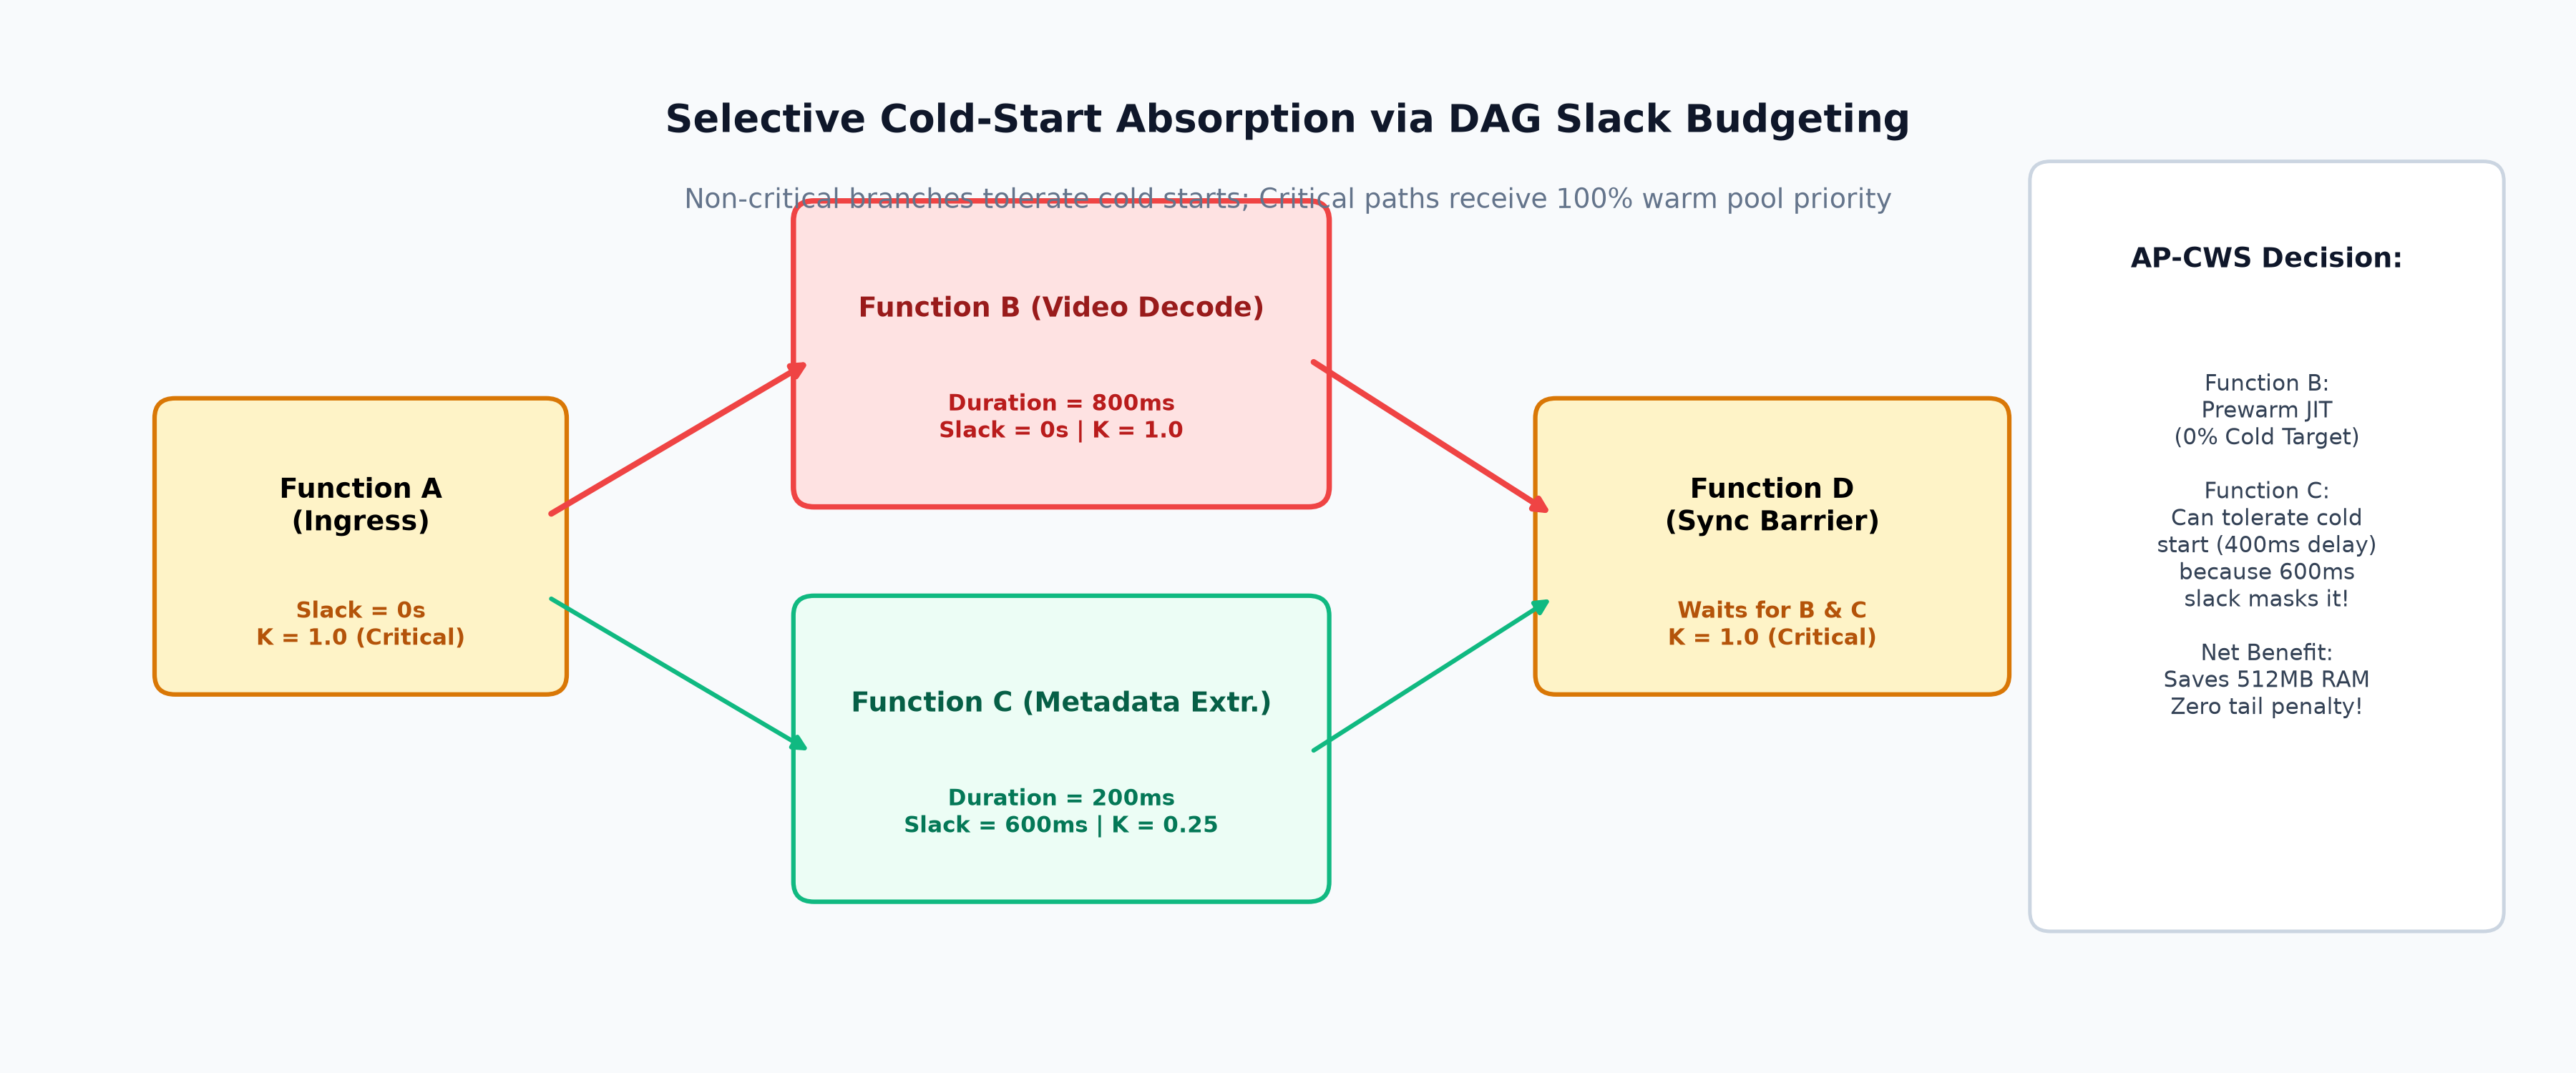
\includegraphics[width=\columnwidth]{diagram1_topological_slack.png}
\vspace{4pt}
\caption{Topological Slack and Criticality Differentiation in Serverless DAG Workflows. Function $f_A$ lies on the zero-slack critical execution path where container initialization delays directly inflate overall workflow completion time. In contrast, parallel task $f_B$ possesses execution slack, which absorbs cold-start latency without impacting workflow completion time.}
\label{fig:diagram1}
\end{figure}

Existing serverless management platforms fail to address this structural distinction. Standard commercial platforms implement fixed keep-alive timeouts, holding idle containers in memory for 10 to 15 minutes after invocation~\cite{shahrad2020serverless}. This static policy ignores incoming traffic trends and DAG dependencies, causing excessive memory consumption during idle periods and frequent cold starts during traffic spikes.

Recent academic approaches attempt to mitigate cold starts by using predictive resource provisioning. The state-of-the-art scheduler proposed by Pan et al.~\cite{pan2024sustainable}, termed SSC, decouples resource management into two isolated stages. Initially, SSC sizes warm container pools according to aggregate call frequencies using an invocation gradient. It subsequently identifies the DAG critical path to guide CPU and memory allocation.

This decoupled architecture contains three fundamental flaws:
1) \textit{Criticality-Agnostic Pool Sizing:} The prewarming stage treats all functions identically. It provisions warm containers for high-slack tasks based purely on request frequency, squandering memory on tasks whose startup delays do not affect workflow latency.
2) \textit{Cold-Start-Agnostic Critical Path:} The scheduling stage computes the critical path assuming deterministic baseline execution times. It ignores the probability that a cold start will double a task's duration and shift the critical path dynamically.
3) \textit{Locality-Unaware Placement:} Placement logic chooses nodes based on CPU and memory availability, not where warm containers are located. Critical tasks get assigned to cold nodes, leading to avoidable startup delays.

To resolve these limitations, this paper proposes AP-CWS (Aware-Predictive Cold-Start Workflow Scheduler). AP-CWS unifies demand forecasting, topological slack budgeting, warm pool sizing, and function placement into a joint optimization framework. Table~\ref{tab:notation} summarizes the mathematical notations and operational definitions used throughout this formulation.

The primary contributions of this work are as follows:
1) \textit{Topological Criticality Metric:} We formulate an analytic criticality index, $K_i \in [0, 1]$, derived from forward and backward topological passes over the workflow DAG~\cite{topcuoglu2002heft}. This index quantifies execution slack and assigns cold-start probability budgets proportionally to task urgency.
2) \textit{Joint Dual-Loop Scheduling Framework:} We implement a dual-loop architecture. A periodic planning loop (running every 60~s) forecasts invocation demand using Holt linear exponential smoothing~\cite{holt2004forecasting} and sizes node-level warm pools. An event-driven dispatch loop places arriving tasks using a multi-factor scoring function that balances container warmth, node performance, and execution cost.
3) \textit{Just-In-Time (JIT) Successor Prewarming:} When a critical task starts execution, the scheduler proactively triggers container initialization for its critical successors on the target node. This mechanism overlaps container startup latency with parent execution time, eliminating critical-path cold starts.
4) \textit{Scalable Fast-AP-CWS Variant:} For high-throughput clusters, we design Fast-AP-CWS. By memoizing DAG structural metrics and evaluating placement candidates using a Power-of-Two-Choices ($d=2$) sub-sampling strategy~\cite{mitzenmacher2001power}, Fast-AP-CWS reduces dispatch overhead from $O(|\mathcal{J}|)$ to $O(1)$.
5) \textit{Extensive Empirical Validation:} We benchmark AP-CWS and Fast-AP-CWS against contemporary baselines across 324 simulation runs using realistic Azure workload traces. We also provide a breaking-point stress test that characterizes queueing saturation and memory collapse under heavy load.

\begin{table*}[t]
\centering
\caption{Comparative Taxonomy of Evaluated Serverless Scheduling Baselines}
\label{tab:baselines}
\footnotesize
\setlength{\tabcolsep}{5pt}
\renewcommand{\arraystretch}{1.18}
\resizebox{\textwidth}{!}{%
\begin{tabular}{p{2.6cm} p{1.6cm} p{2.2cm} p{2.2cm} p{2.2cm} p{2.0cm} p{5.5cm}}
\toprule
\rowcolor{tableheader}
\textbf{Reference \& Venue} & \textbf{Evaluated Baseline} & \textbf{Optimization Objective} & \textbf{Prewarming Strategy} & \textbf{DAG Structural Awareness} & \textbf{Task-Node Placement Coupling} & \textbf{Core Algorithmic Limitation} \\
\midrule
Shahrad et al., \textit{USENIX ATC '20}~\cite{shahrad2020serverless} & Fixed 10-Min Keep-Alive & Minimize startup frequency & Fixed 10-minute idle container retention & None (Independent function invocations) & Decoupled (Default greedy bin-packing) & Keeps idle containers regardless of future demand; causes memory exhaustion during load spikes. \\
\rowcolor{tablerowalt}
Pan et al., \textit{IEEE T-SUSC '24}~\cite{pan2024sustainable} (Base Paper) & SSC & Minimize dollar cost and makespan & Frequency gradient trend extrapolation & Critical path used only for CPU/RAM sizing & Decoupled (Sequential independent stages) & Sizes pools without topological slack; places critical tasks without checking warm container locality. \\
Chen et al., \textit{FGCS '25}~\cite{chen2025casr} & CASR & Reduce cold starts under cache limits & Frequency-recency caching (W-TinyLFU~\cite{einziger2017tinylfu}) & None (Local container eviction) & Decoupled (Host-local container cache) & Evicts infrequent intermediate join tasks; creates cascading tail delays at workflow barriers. \\
\rowcolor{tablerowalt}
Nguyen et al., \textit{MASCOTS '25}~\cite{nguyen2025mpc} & MPC & Minimize cold starts under memory bounds & Rolling-horizon queue deferral and prewarm & None (Applies to isolated function queues) & Decoupled (Centralized memory bounds) & Request deferral introduces artificial queueing delays that violate strict workflow deadlines. \\
Alquraan et al., \textit{EuroSys '26}~\cite{alquraan2026drops} & DROPS & Bound tail latency under strict SLOs & Quantile-based dynamic pool dimensioning & Weak (End-to-end deadline partitioning) & Decoupled (Cluster-wide reservation) & High-percentile sizing overprovisions idle warm pools; triggers severe memory contention under high concurrency. \\
\rowcolor{highlightgreen}
\textbf{Proposed Work} & \textbf{AP-CWS \& Fast-AP-CWS} & \textbf{Minimize P95 latency, cost, and SLO violations} & \textbf{Topological slack budgeting with JIT prewarming} & \textbf{Full DAG awareness (Dynamic $K_i$ slack tracking)} & \textbf{Fully Coupled (Joint warmth, cost, and speed scoring)} & \textbf{Requires workflow graph definition and periodic matrix updates.} \\
\bottomrule
\end{tabular}%
}
\end{table*}

\section{Related Work}
\label{sec:related}
Serverless cold-start mitigation techniques fall into three operational categories: idle container caching, predictive container prewarming, and DAG workflow scheduling. Table~\ref{tab:baselines} summarizes the baseline approaches evaluated in this work alongside our proposed schedulers.

\subsection{Keep-Alive and Cache-Replacement Baselines}
Industry platforms rely on static keep-alive timers. Shahrad et al.~\cite{shahrad2020serverless} analyzed commercial serverless workloads and found high variance in invocation arrival intervals. Modern platforms retain idle containers for 10 minutes. This heuristic consumes memory without regard for application structure. Fuerst and Sharma developed FaasCache~\cite{fuerst2021faascache}, demonstrating that greedy cache management can retain warm containers effectively for independent functions. Chen et al.~\cite{chen2025casr} introduced CASR, which employs Windowed TinyLFU~\cite{einziger2017tinylfu} to balance recency and frequency in local container pools. While CASR reduces cold starts for frequently invoked leaf functions, it penalizes intermediate synchronization tasks. Hanaforoosh et al.~\cite{hanaforoosh2025granularity} investigated task aggregation via granularity trees to fuse small functions, but this requires manual or static compilation changes. In a DAG workflow, join tasks may experience low invocation frequencies but reside directly on the critical execution path. Evicting these containers introduces synchronization stalls that inflate workflow tail latency.

\subsection{Predictive and Sizing Baselines}
To avoid reactive initialization, predictive methods provision containers ahead of invocations. Nguyen et al.~\cite{nguyen2025mpc} formulated a Model Predictive Control (MPC) strategy. Their approach solves a rolling-horizon optimization problem to smooth container allocations. However, MPC relies on request deferral during transient traffic peaks. Deferring execution inserts queueing delays into time-critical workflows, conflicting directly with contractual Service-Level Objectives. Alquraan et al.~\cite{alquraan2026drops} developed DROPS, using statistical quantile tracking to size container pools for tail demand in Azure Functions. DROPS provisions capacity uniformly across all workflow components. When arrival rates accelerate, this uniform reservation consumes available host memory with idle containers, blocking active task execution and precipitating system thrashing.

\subsection{Workflow-Aware Schedulers}
Scheduling multi-function DAGs requires coordinating task placement across heterogeneous nodes while respecting execution precedence~\cite{li2022faasflow, yu2023pheromone, carver2020wukong, zolfaghari2025dynamic}. Carver et al. implemented Wukong~\cite{carver2020wukong}, a locality-enhanced parallel computing engine for serverless workflows. Li et al. presented FaaSFlow~\cite{li2022faasflow}, which partitions workflows into subgraphs to balance inter-function communication costs against execution latency. Yu et al. proposed Pheromone~\cite{yu2023pheromone}, demonstrating that data-centric coordination avoids centralized scheduler bottlenecks. Zolfaghari et al.~\cite{zolfaghari2025dynamic} investigated multi-objective dynamic placement in edge clusters, focusing on energy and makespan trade-offs.

Our work builds directly upon the baseline of SSC (Pan et al.~\cite{pan2024sustainable}). SSC separates workflow resource management into two disjoint phases. First, it computes invocation frequency gradients to determine prewarm counts. Second, it identifies the DAG critical path to size CPU and memory allocations.

This decoupling produces sub-optimal allocations. SSC sizes warm pools without determining whether a function possesses execution slack. As a result, physical memory is allocated to non-critical tasks that could tolerate cold starts without increasing workflow makespan. In addition, SSC assigns tasks using greedy resource metrics without verifying container warmth on candidate nodes, frequently dispatching critical-path tasks to cold hosts. AP-CWS directly resolves these weaknesses by unifying slack-based probability budgeting, warm-aware placement scoring, and Just-In-Time successor prewarming into a single framework.

\section{System, Network, and Energy Node Models}
\label{sec:system}

\subsection{Heterogeneous Serverless Cluster Architecture}
We model a serverless compute cluster managed by a centralized control plane. The cluster consists of a set of heterogeneous worker nodes denoted by $\mathcal{J} = \{1, 2, \dots, M\}$. Each worker node $j \in \mathcal{J}$ possesses physical hardware specifications characterized by:
1) $C_j$: Total processing capacity expressed in normalized CPU cores.
2) $M_j$: Total physical memory capacity measured in megabytes (MB).
3) $v_j$: Relative execution speed factor. A node with $v_j = 1.2$ completes computational cycles 20\% faster than a baseline node ($v = 1.0$).
4) $p_j$: Unit financial cost per gigabyte-hour (\$/GB-hr) for active resource allocation.

Each worker node runs a local container daemon that manages container lifecycles. Nodes maintain two distinct pools of memory: active memory allocated to currently executing function instances, and warm memory reserved for idle containers awaiting invocation.

\subsection{Container Lifecycle and Execution State Machine}
A function $f_i$ requires a memory footprint of $m_i$~MB and an allocated CPU share of $c_i$ cores. When function $f_i$ is dispatched to node $j$, the node container manager transitions through an explicit state machine:
1) \textit{State 0 (Uninstantiated):} No container image or runtime sandbox for $f_i$ exists in memory on node $j$.
2) \textit{State 1 (Cold Initialization):} If no warm container is available, node $j$ cold starts. The node pulls the container image, configures cgroups and namespaces, and launches the runtime environment. This phase incurs a cold-start delay $s_i$.
3) \textit{State 2 (Active Execution):} The container executes function logic. The actual run time $t_{ij}$ depends on the function's base duration $t_i^{base}$ on a reference node and the node speed factor $v_j$:
\begin{equation}
    t_{ij} = \frac{t_i^{base}}{v_j}
\end{equation}
4) \textit{State 3 (Idle Warm Keep-Alive):} After execution completes, the container does not terminate right away. It transitions to an idle warm state, retaining its memory allocation $m_i$ on node $j$. If another invocation for $f_i$ arrives before the keep-alive window expires, the task runs immediately with zero startup delay.
5) \textit{State 4 (Eviction):} If the keep-alive timer expires, or the node needs physical memory to service a higher-priority invocation, the container terminates, returning $m_i$ to the free memory pool.

\subsection{Network Communication Model}
In a serverless workflow, dependencies between parent function $f_i$ and child function $f_k$ necessitate transmitting intermediate output payloads. Let $d_{ik}$ denote the size of the intermediate data payload in MB.

Communication delay $\tau_{ik}^{net}$ between node $j$ (executing $f_i$) and node $j'$ (executing $f_k$) depends on placement locality:
\begin{equation}
\tau_{ik}^{net}(j, j') = \begin{cases} 
0, & \text{if } j = j' \\ 
\frac{d_{ik}}{B_{net}} + \delta_{prop}, & \text{if } j \neq j' 
\end{cases}
\end{equation}
where $B_{net}$ is the cluster interconnect bandwidth (e.g., 10~Gbps) and $\delta_{prop}$ is the base network propagation latency. Co-locating parent and child tasks on the same physical node eliminates network serialization and transfer latency.

\subsection{Energy and Resource Consumption Model}
The energy consumption of node $j$ over an operational time interval $\Delta$ is composed of baseline static power, active execution power, cold-start initialization power, and idle memory retention power:
\begin{equation}
\begin{aligned}
E_j(\Delta) = & P_j^{idle} \cdot \Delta + \sum_{f_i \in \mathcal{A}_j} P_{ij}^{exec} \cdot t_{ij} \\
& + \sum_{f_i \in \mathcal{C}_j} P_{ij}^{cold} \cdot s_i + \sum_{f_i \in \mathcal{W}_j} P_j^{mem} \cdot m_i \cdot \Delta_i^{warm}
\end{aligned}
\end{equation}
where $P_j^{idle}$ is baseline static idle power, $P_{ij}^{exec}$ is dynamic CPU computation power, $P_{ij}^{cold}$ is startup burst power, and $P_j^{mem}$ is memory refresh power per MB-hour. Sets $\mathcal{A}_j$, $\mathcal{C}_j$, and $\mathcal{W}_j$ represent active tasks, cold-started tasks, and warm-retained containers on node $j$, respectively.

This formulation captures the fundamental system trade-off: retaining warm containers expends continuous DRAM refresh energy, whereas excessive cold starts induce CPU power spikes and lengthen task makespans. A well-designed scheduler must coordinate these competing objectives.

\section{Problem Formulation}
\label{sec:formulation}

\subsection{Workflow DAG Representation}
We represent a serverless workflow application as a Directed Acyclic Graph $\mathcal{G} = (\mathcal{V}, \mathcal{E})$, where:
1) $\mathcal{V} = \{f_1, f_2, \dots, f_N\}$ is the set of $N$ constituent serverless functions.
2) $\mathcal{E} \subseteq \mathcal{V} \times \mathcal{V}$ is the set of directed edges representing execution precedence and data dependencies. An edge $(f_i, f_k) \in \mathcal{E}$ indicates that child function $f_k$ cannot begin execution until parent function $f_i$ completes and delivers its output data.

Each workflow has defined entry functions $\mathcal{V}_{entry} = \{f \in \mathcal{V} \mid \text{parents}(f) = \emptyset\}$ and exit functions $\mathcal{V}_{exit} = \{f \in \mathcal{V} \mid \text{children}(f) = \emptyset\}$. The application is governed by an end-to-end Service Level Objective deadline, denoted by $T_{SLO}$. Fig.~\ref{fig:diagram2} illustrates the structural topologies and deadline configurations of the evaluated serverless workflow benchmark pipelines.

\begin{figure*}[t]
\centering
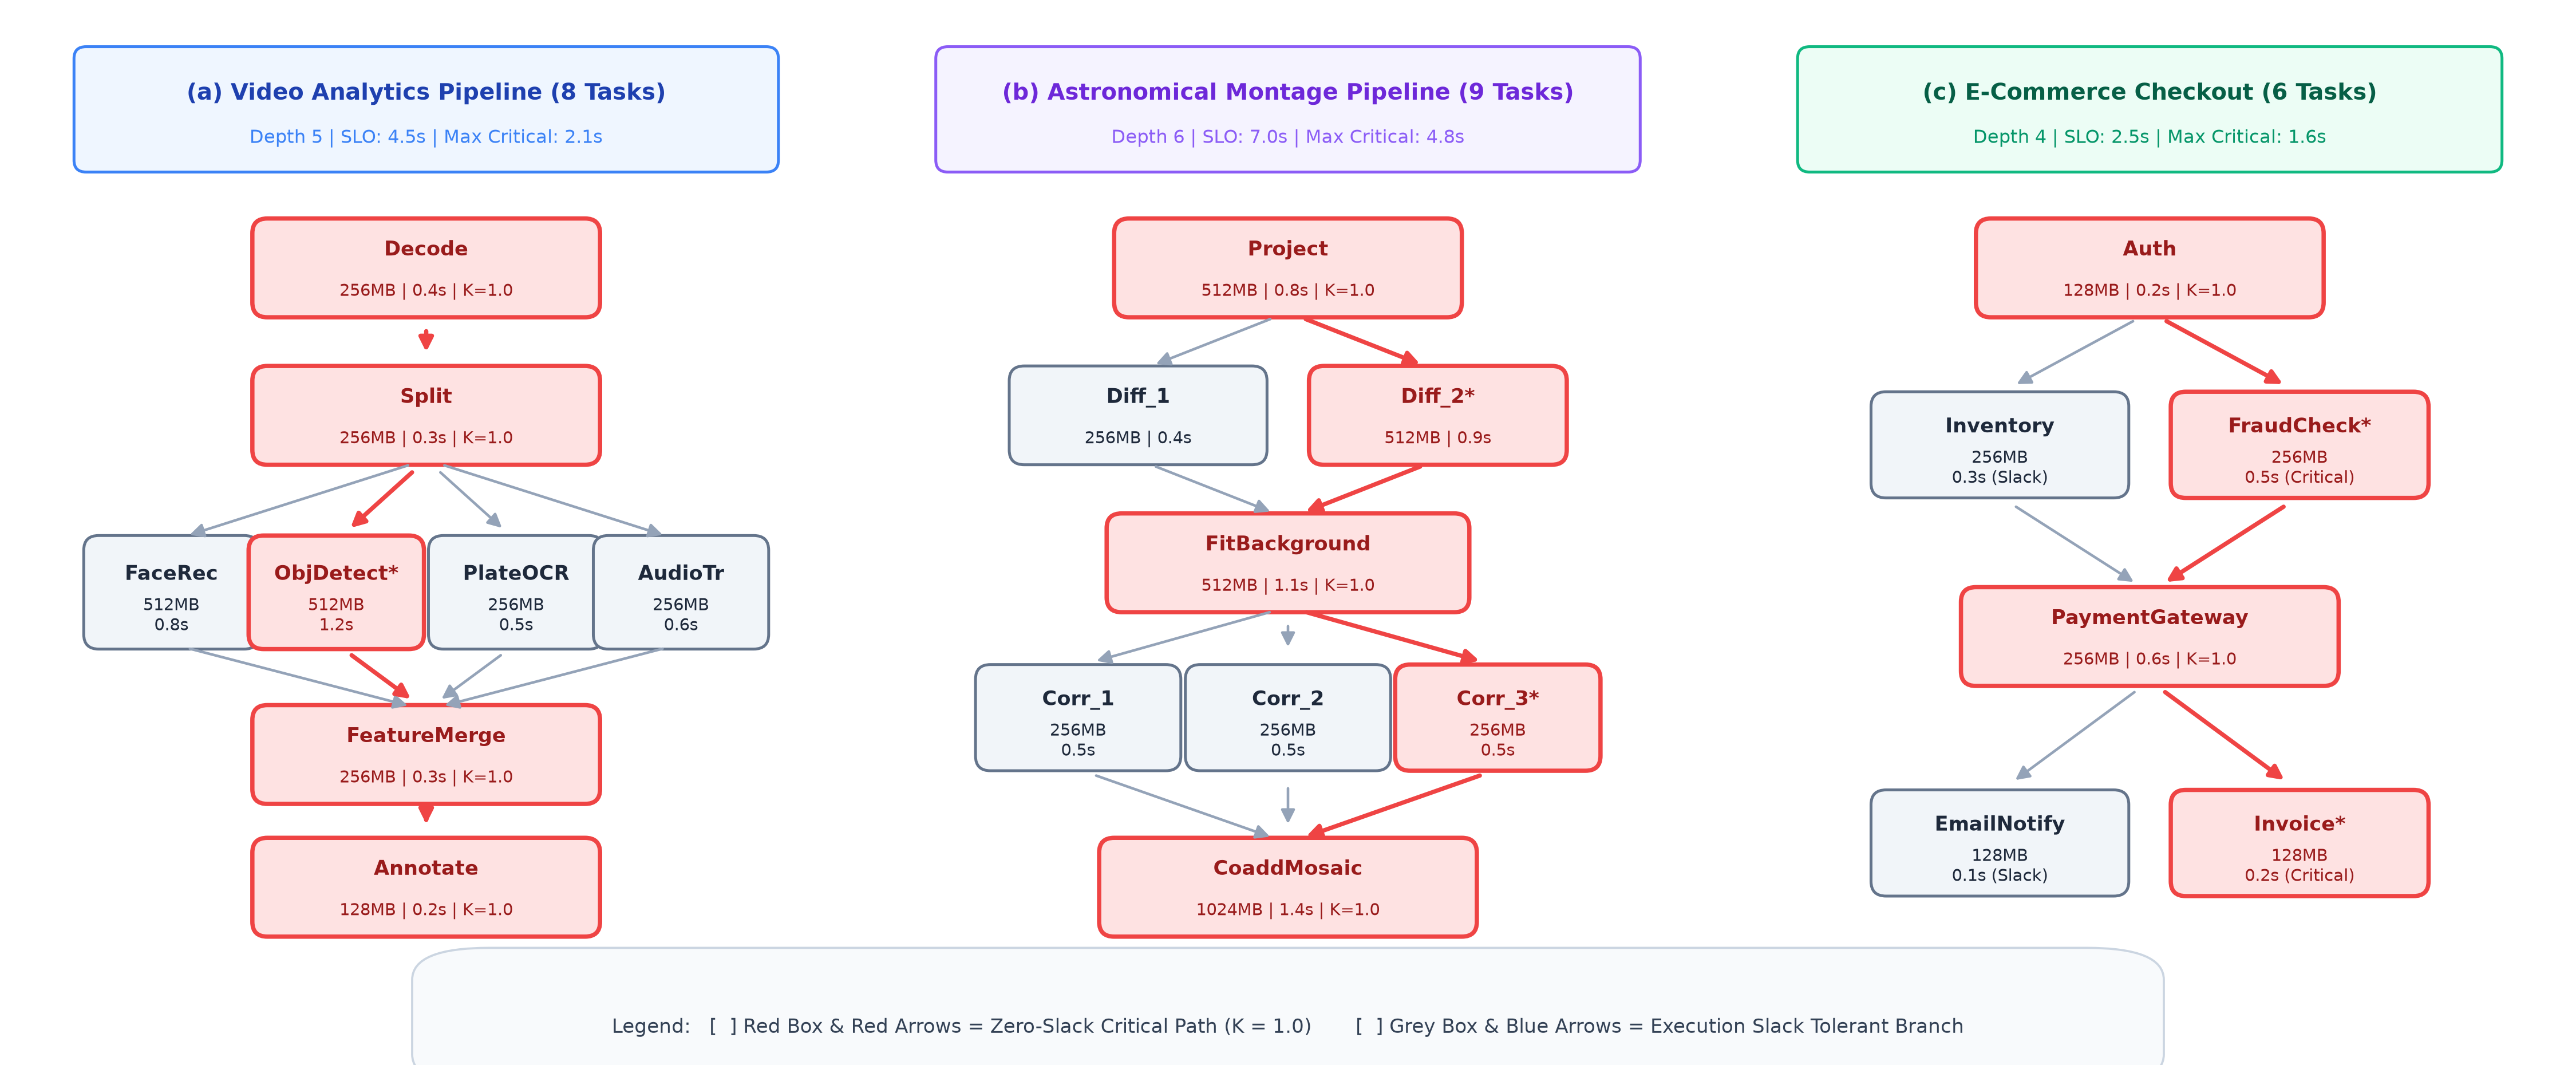
\includegraphics[width=0.82\textwidth]{diagram2_workflow_topologies.png}
\vspace{4pt}
\caption{Structural Topologies of Evaluated Serverless Workflow Benchmarks: (a) Video Analytics Pipeline (8 functions, depth 5, deadline 4.5~s), (b) Astronomical Montage Pipeline~\cite{deelman2005pegasus} (9 functions, depth 6, deadline 7.0~s), and (c) E-Commerce Transaction Pipeline (6 functions, depth 4, deadline 2.5~s). Asterisks and bold red paths mark zero-slack critical execution sequences.}
\label{fig:diagram2}
\end{figure*}

\subsection{Topological Timing Analysis and Slack Budgeting}
To quantify execution flexibility across the graph, the scheduler performs forward and backward topological passes based on classical list scheduling principles~\cite{topcuoglu2002heft}:
1) \textit{Earliest Start Time ($EST$):} The earliest time a function can start executing, assuming all predecessor tasks execute without delay:
\begin{equation}
EST(f_i) = \begin{cases} 
0, & \text{if } f_i \in \mathcal{V}_{entry} \\ 
\max\limits_{f_p \in \text{par}(f_i)} (EST(f_p) + \bar{t}_p), & \text{otherwise} 
\end{cases}
\end{equation}
where $\bar{t}_p$ is the expected execution duration of parent task $f_p$ on a baseline node, and $\text{par}(f_i)$ denotes the set of immediate parent functions.
2) \textit{Earliest Finish Time ($EFT$):}
\begin{equation}
EFT(f_i) = EST(f_i) + \bar{t}_i
\end{equation}
3) \textit{Workflow Minimum Makespan ($T^*$):}
\begin{equation}
T^* = \max_{f_e \in \mathcal{V}_{exit}} EFT(f_e)
\end{equation}
4) \textit{Latest Finish Time ($LFT$):} The last moment a function can finish without delaying the entire workflow past $T^*$:
\begin{equation}
LFT(f_i) = \begin{cases} 
T^*, & \text{if } f_i \in \mathcal{V}_{exit} \\ 
\min\limits_{f_c \in \text{ch}(f_i)} (LST(f_c)), & \text{otherwise} 
\end{cases}
\end{equation}
where $\text{ch}(f_i)$ represents immediate child tasks.
5) \textit{Latest Start Time ($LST$):}
\begin{equation}
LST(f_i) = LFT(f_i) - \bar{t}_i
\end{equation}
6) \textit{Topological Slack ($\text{Slack}_i$):} Spare execution buffer for function $f_i$:
\begin{equation}
\text{Slack}_i = LST(f_i) - EST(f_i)
\end{equation}

Tasks with $\text{Slack}_i = 0$ constitute the critical execution path of the workflow.

\subsection{Topological Criticality Formulation}
For each function $f_i$, we define the normalized criticality index $K_i$ as:
\begin{equation}
K_i = 1 - \frac{\text{Slack}_i}{T^*}
\end{equation}
Because $0 \le \text{Slack}_i \le T^*$, the criticality index is strictly bounded: $0 \le K_i \le 1$.
1) When $K_i = 1.0$: Function $f_i$ has zero slack and is directly on the critical path. Any cold start on $f_i$ directly increases overall workflow completion time.
2) When $K_i \to 0$: Function $f_i$ has substantial execution slack. A cold start on $f_i$ will be absorbed by the slack buffer, having zero impact on end-to-end latency.

\subsection{Decision Variables}
The scheduling system controls two primary sets of decision variables:
1) $W_{ij} \in \mathbb{Z}_{\ge 0}$: Number of warm container instances for function $f_i$ on node $j$ during planning epoch $\Delta$.
2) $x_{ij} \in \{0, 1\}$: Binary placement indicator, where $x_{ij} = 1$ if task instance $f_i$ is dispatched to node $j$, and $0$ otherwise.
3) $y_{ij} \in \{0, 1\}$: Binary startup indicator, where $y_{ij} = 0$ if task $f_i$ finds an idle warm container on node $j$, and $y_{ij} = 1$ if it incurs a cold start.

\subsection{Optimization Objectives and Constraints}
The scheduling problem seeks to optimize three conflicting criteria: tail latency, cold-start rate, and monetary resource cost.
1) \textit{P95 Workflow Completion Time ($T_{P95}$):}
\begin{equation}
\min \quad T_{P95}(\mathcal{G})
\end{equation}
where $T(\mathcal{G}) = \max_{f_e \in \mathcal{V}_{exit}} \left( t_e^{start} + t_{ej} + y_{ej} \cdot s_e \right)$.
2) \textit{Critical-Path Cold-Start Rate ($R_{crit}$):}
\begin{equation}
\min \quad R_{crit} = \frac{\sum_{f_i \in \mathcal{V}} K_i \cdot y_{ij}}{\sum_{f_i \in \mathcal{V}} K_i}
\end{equation}
3) \textit{Total Monetary Cost ($C_{total}$):}
\begin{equation}
\begin{aligned}
\min \quad C_{total} = \sum_{j \in \mathcal{J}} p_j \Bigg( & \sum_{f_i \in \mathcal{V}} x_{ij} \frac{m_i t_{ij}}{1024 \cdot 3600} \\
& + \sum_{f_i \in \mathcal{V}} W_{ij} \frac{m_i \Delta}{1024 \cdot 3600} \Bigg)
\end{aligned}
\end{equation}

Subject to the following operational constraints:
1) \textit{Precedence Constraint:} For every edge $(f_i, f_k) \in \mathcal{E}$:
\begin{equation}
t_k^{start} \ge t_i^{finish} + \tau_{ik}^{net}(j, j'), \quad \forall (f_i, f_k) \in \mathcal{E}
\end{equation}
2) \textit{Node Memory Limit:} At any point in time $t$:
\begin{equation}
\sum_{f_i \in \mathcal{A}_j(t)} m_i + \sum_{f_i \in \mathcal{V}} W_{ij} \cdot m_i \le M_j, \quad \forall j \in \mathcal{J}
\end{equation}
3) \textit{Node CPU Capacity Constraint:} Active CPU utilization on node $j$ must not exceed total physical cores $C_j$:
\begin{equation}
\sum_{f_i \in \mathcal{A}_j(t)} c_i \le C_j, \quad \forall j \in \mathcal{J}
\end{equation}
4) \textit{Unique Assignment Constraint:} Every task invocation must be assigned to exactly one worker node:
\begin{equation}
\sum_{j \in \mathcal{J}} x_{ij} = 1, \quad \forall f_i \in \mathcal{V}
\end{equation}
5) \textit{SLO Compliance Constraint:} Total workflow completion time should satisfy the target deadline:
\begin{equation}
T(\mathcal{G}) \le T_{SLO}
\end{equation}

Because exact optimization of this NP-hard combinatorial formulation is computationally intractable under sub-second serverless latency constraints, practical execution demands an efficient heuristic approach. Sections~\ref{sec:planning} and~\ref{sec:dispatch} detail our dual-loop framework and its constant-time hyperscale variant.

\section{Proposed Approach}
\label{sec:approach}
This paper introduces AP-CWS (Aware-Predictive Cold-Start Workflow Scheduler), a unified resource scheduling framework for serverless DAG workflows. AP-CWS coordinates warm container pool dimensioning and task placement through two cooperating control loops:
1) \textit{Periodic Offline Planning Loop:} Runs at regular intervals ($\Delta = 60\text{ s}$) to forecast function invocation rates, compute topological slack budgets, and determine target warm pool sizes per cluster node.
2) \textit{Event-Driven Online Dispatch Loop:} Runs on every function invocation. Computes joint placement scores across candidate nodes and triggers JIT container prewarming for critical successor functions.

In addition, we formulate Fast-AP-CWS, a high-throughput variant for hyperscale clusters with unpredictable, high-frequency request arrivals. Fig.~\ref{fig:diagram3} shows the overall two-phase scheduling architecture of AP-CWS, detailing the interaction between the periodic planning cycle and the event-driven dispatch loop.

\begin{figure*}[t]
\centering
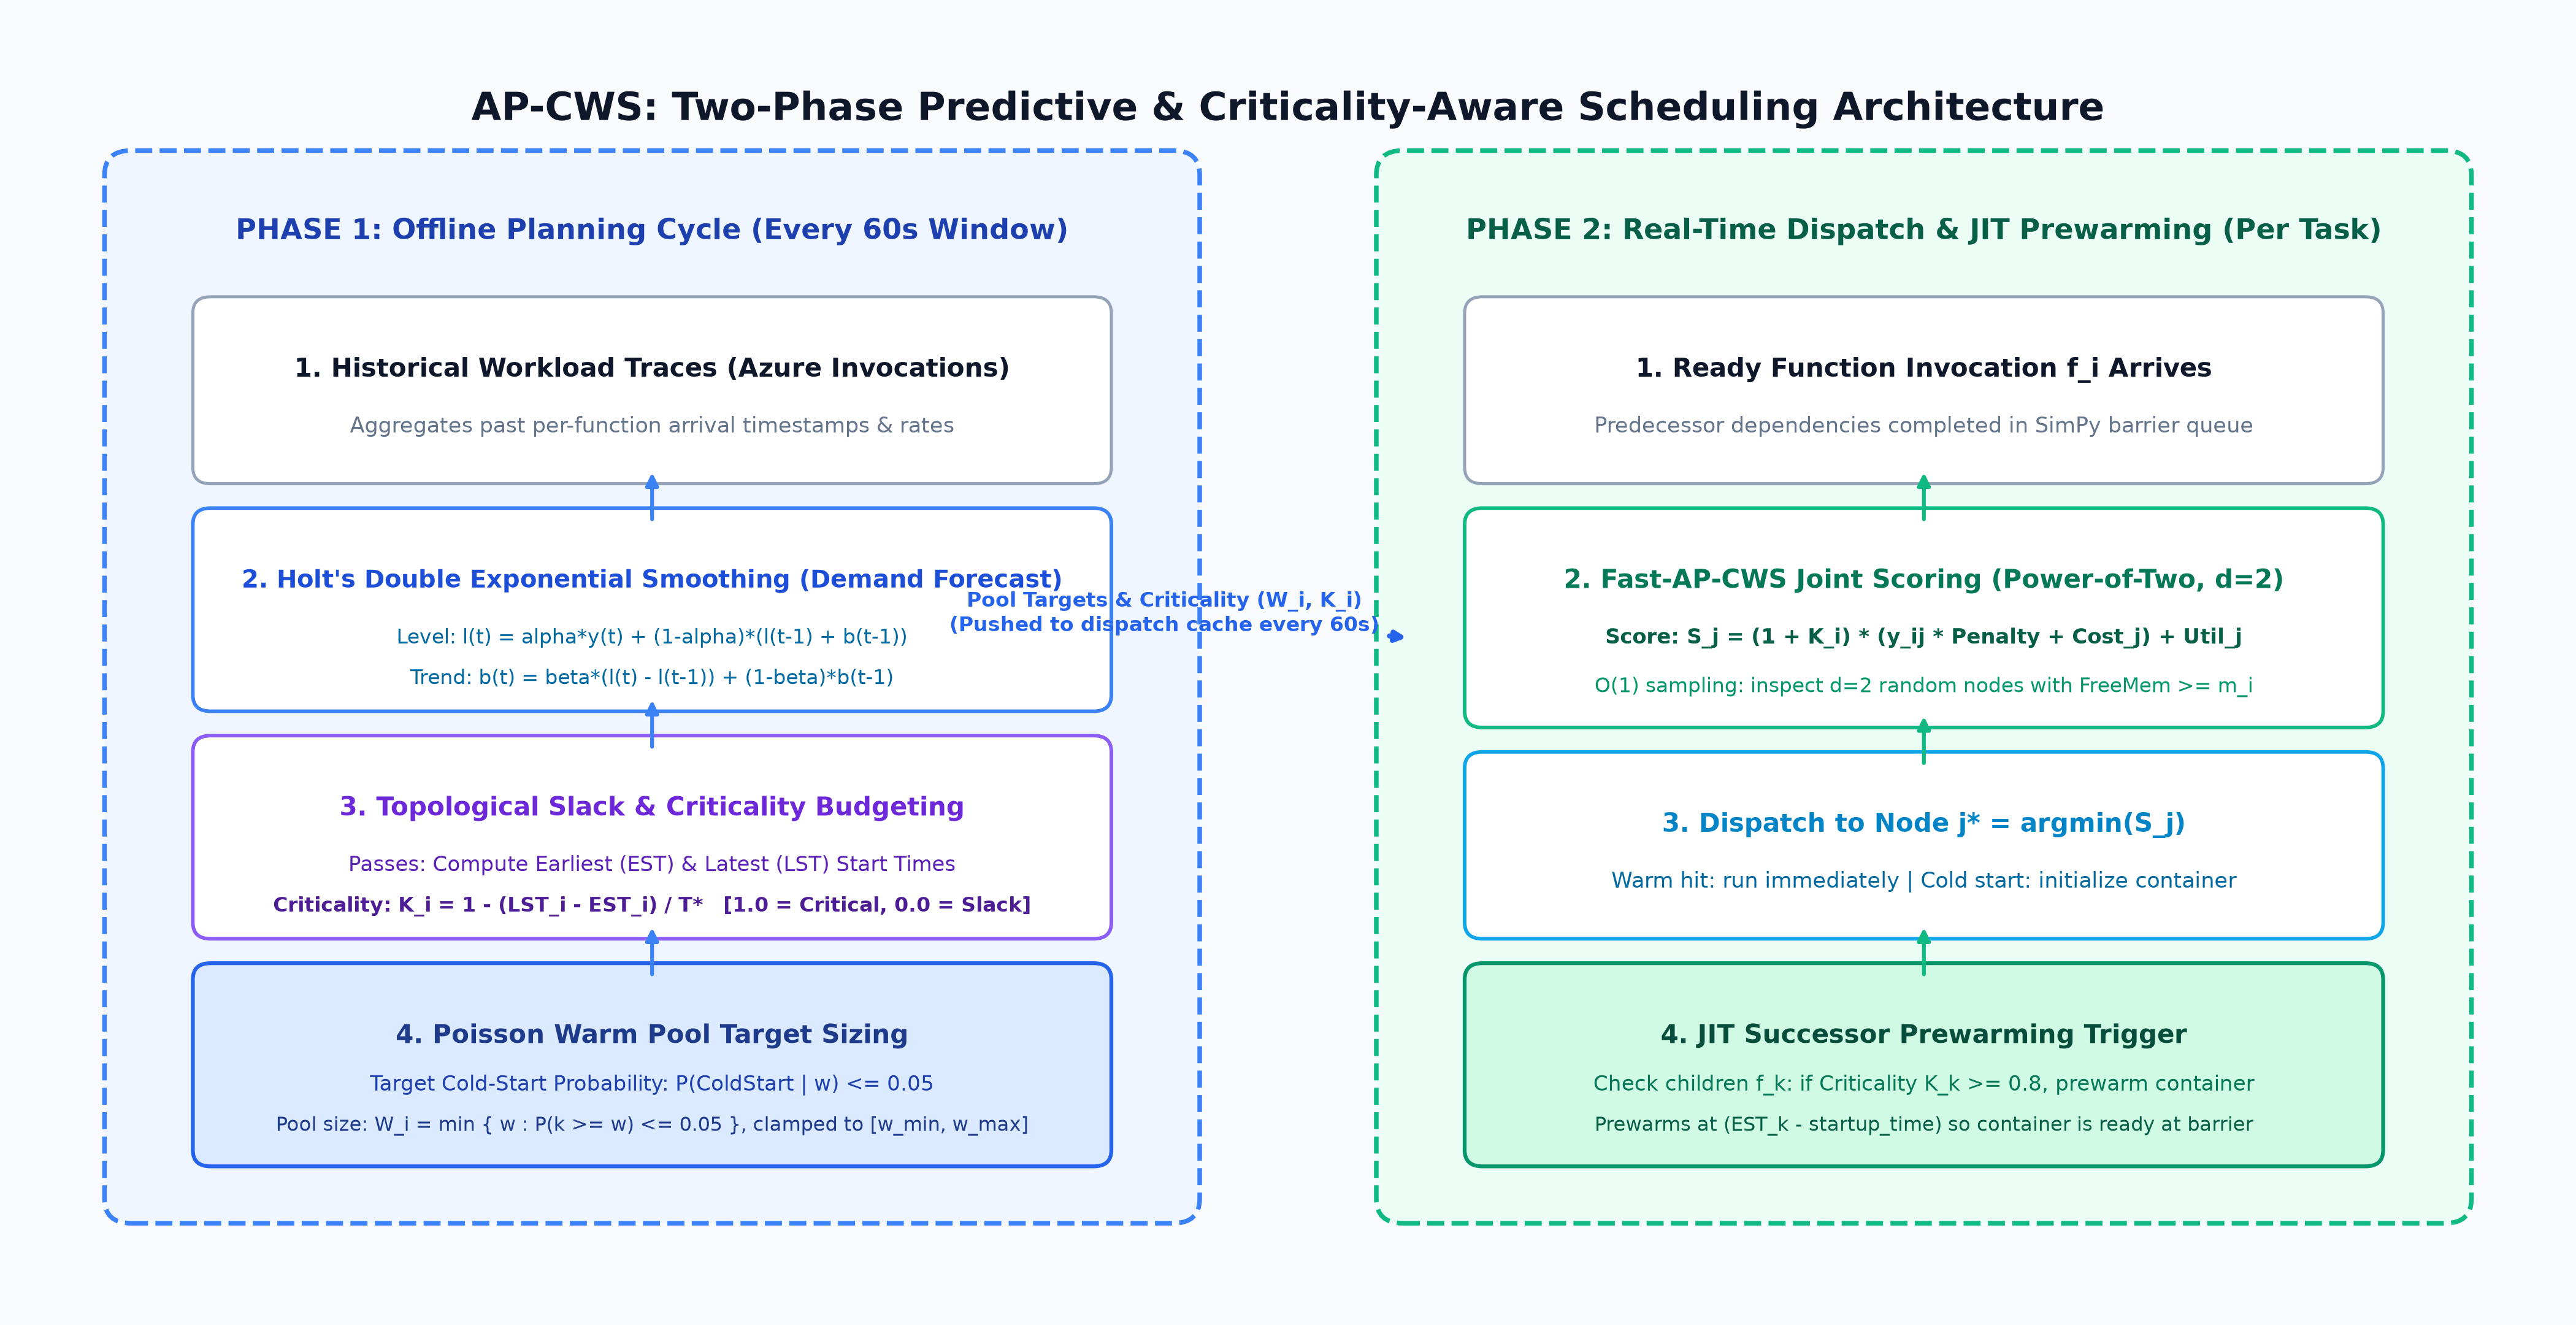
\includegraphics[width=0.84\textwidth]{diagram3_architecture.png}
\vspace{4pt}
\caption{AP-CWS Two-Phase Predictive and Criticality-Aware Scheduling Architecture. The periodic planning loop (left) updates demand forecasts via Holt smoothing and dimensions warm container pools based on topological slack budgets. The event-driven dispatch loop (right) places incoming tasks using joint scoring and triggers Just-In-Time successor prewarming on target execution nodes.}
\label{fig:diagram3}
\end{figure*}

\subsection{Periodic Planning Loop: Slack Budgeting and Warm Pool Sizing}
\label{sec:planning}
The planning loop runs every $\Delta$ seconds. It determines how many warm containers each function requires to bound cold starts.

\subsubsection{Demand Forecasting via Holt Linear Exponential Smoothing}
Function arrival patterns show short-term trends and time-of-day shifts. Standard moving averages react too slowly to traffic surges, while higher-order autoregressive models incur excessive computational overhead. We use Holt linear exponential smoothing~\cite{holt2004forecasting} to estimate the invocation arrival rate $\hat{\lambda}_i$ for each function $f_i \in \mathcal{V}$.

Let $Y_t$ be the observed invocation count of function $f_i$ during planning epoch $t$. The forecast updates the smoothed level $L_t$ and trend $T_t$:
\begin{equation}
L_t = \alpha Y_t + (1 - \alpha)(L_{t-1} + T_{t-1})
\end{equation}
\begin{equation}
T_t = \beta (L_t - L_{t-1}) + (1 - \beta) T_{t-1}
\end{equation}
where $\alpha \in [0, 1]$ is the data smoothing factor and $\beta \in [0, 1]$ is the trend smoothing factor. In our implementation, we configure $\alpha = 0.2$ and $\beta = 0.1$. The projected invocation rate for the next epoch is:
\begin{equation}
\hat{\lambda}_i = \frac{\max(0, L_t + T_t)}{\Delta}
\end{equation}

\subsubsection{Topological Criticality and Cold-Start Probability Budgeting}
Topological slack indicates how much delay a function can tolerate without postponing workflow completion. Using minimum makespan $T^*$ and slack $\text{Slack}_i = LST(f_i) - EST(f_i)$, the scheduler computes $K_i = 1 - (\text{Slack}_i / T^*)$.

Prior schedulers allocate warm containers uniformly. In contrast, AP-CWS maps criticality to an allowable cold-start probability budget, denoted by $p_i^{target}$:
\begin{equation}
p_i^{target} = (1 - K_i) \cdot p_{max} + \epsilon
\end{equation}
where $p_{max} = 0.50$ is maximum tolerable cold-start probability for slack tasks, and $\epsilon = 0.01$ is baseline tolerance.
1) When $K_i = 1.0$ (critical path), $p_i^{target} = \epsilon = 0.01$, enforcing a strict 1\% cold-start ceiling.
2) When $K_i \to 0$ (parallel branch), $p_i^{target} \approx 0.51$, permitting cold starts since slack absorbs startup delays.

\subsubsection{Analytic Pool Sizing Inversion}
Assuming function invocations follow an arrival process with rate $\hat{\lambda}_i$ and average warm execution duration $\bar{t}_i$, the probability of a cold start given a warm pool size of $W_i$ instances is modeled as:
\begin{equation}
P(W_i) = \exp\left( -\frac{\hat{\lambda}_i \cdot \bar{t}_i + \delta}{W_i + 1} \right)
\end{equation}
where $\delta > 0$ prevents division by zero. Inverting the model to ensure $P(W_i) \le p_i^{target}$ yields:
\begin{equation}
W_i^* = \left\lceil -\frac{\hat{\lambda}_i \cdot \bar{t}_i + \delta}{\ln(p_i^{target})} \right\rceil
\end{equation}

The scheduler clamps $W_i^*$ to $[W_{min}, W_{max}]$. For critical tasks ($K_i \ge 0.8$), $W_{min} = 1$ ensures at least one warm container remains allocated.

\subsubsection{Cluster Warm Pool Placement}
Once total warm capacity $W_i$ is determined, instances are packed onto nodes in descending order of criticality $K_i$, prioritizing nodes with higher speed factors $v_j$ and unreserved memory $M_j^{free} \ge m_i$.

\subsection{Event-Driven Dispatch Loop: Joint Scoring and JIT Prewarming}
\label{sec:dispatch}

\subsubsection{Multi-Factor Placement Scoring Function}
The scheduler evaluates candidate worker nodes using a joint placement score $S_{ij}$:
\begin{equation}
\begin{aligned}
S_{ij} = & (1 + K_i) \left[ y_{ij} \left( \frac{s_i}{v_j} \right) + \frac{t_i^{base}}{v_j} \right] \\
& + \mu p_j \left( \frac{m_i}{1024} \right) - \gamma \left( \frac{M_j^{free}}{M_j} \right)
\end{aligned}
\end{equation}
where $y_{ij} \in \{0, 1\}$ indicates container status ($0$ if warm, $1$ if cold), $s_i / v_j$ is node-scaled startup delay, $t_i^{base} / v_j$ is execution duration, $p_j$ is hourly price ($\mu = 0.05$), and $M_j^{free} / M_j$ is normalized headroom ($\gamma = 0.10$).

The weighting factor $(1 + K_i)$ amplifies the latency penalty for critical tasks. When $f_i$ lies on the critical path ($K_i = 1.0$), cold-start penalties and execution delays are doubled in the scoring metric, directing the scheduler toward warm, high-speed nodes even if hourly rate $p_j$ is higher. In contrast, when $f_i$ possesses substantial slack ($K_i \to 0$), the delay weight shrinks, allowing monetary cost considerations to steer placement toward lower-cost nodes.

The target node $j^*$ is chosen by minimizing the score:
\begin{equation}
j^* = \arg\min_{j \in \mathcal{J}, M_j^{free} \ge m_i} S_{ij}
\end{equation}

\subsubsection{Proactive Just-In-Time (JIT) Successor Prewarming}
To eliminate cascading delays, AP-CWS implements JIT successor prewarming. When task $f_i$ begins executing on node $j^*$, the scheduler inspects its immediate child tasks $f_k \in \text{children}(f_i)$.

If child task $f_k$ satisfies the criticality threshold $K_k \ge \kappa$ ($\kappa = 0.60$) and node $j^*$ lacks an idle warm container for $f_k$, an asynchronous prewarm signal is dispatched to node $j^*$. Because parent execution $t_{ij^*}$ overlaps with child initialization delay $s_k$:
\begin{equation}
t_{overlap} = \min(t_{ij^*}, s_k)
\end{equation}
startup delay drops from $s_k$ to $\max(0, s_k - t_{ij^*})$. When parent $f_i$ completes, child $f_k$ executes immediately on the warm instance with zero network delay ($\tau_{ik}^{net} = 0$).

\subsection{Operational Modes: AP-CWS vs. Fast-AP-CWS}
As contrasted in Fig.~\ref{fig:diagram4}, AP-CWS supports two operational regimes tailored to different cluster scales and arrival intensities.

\begin{figure*}[!t]
\centering
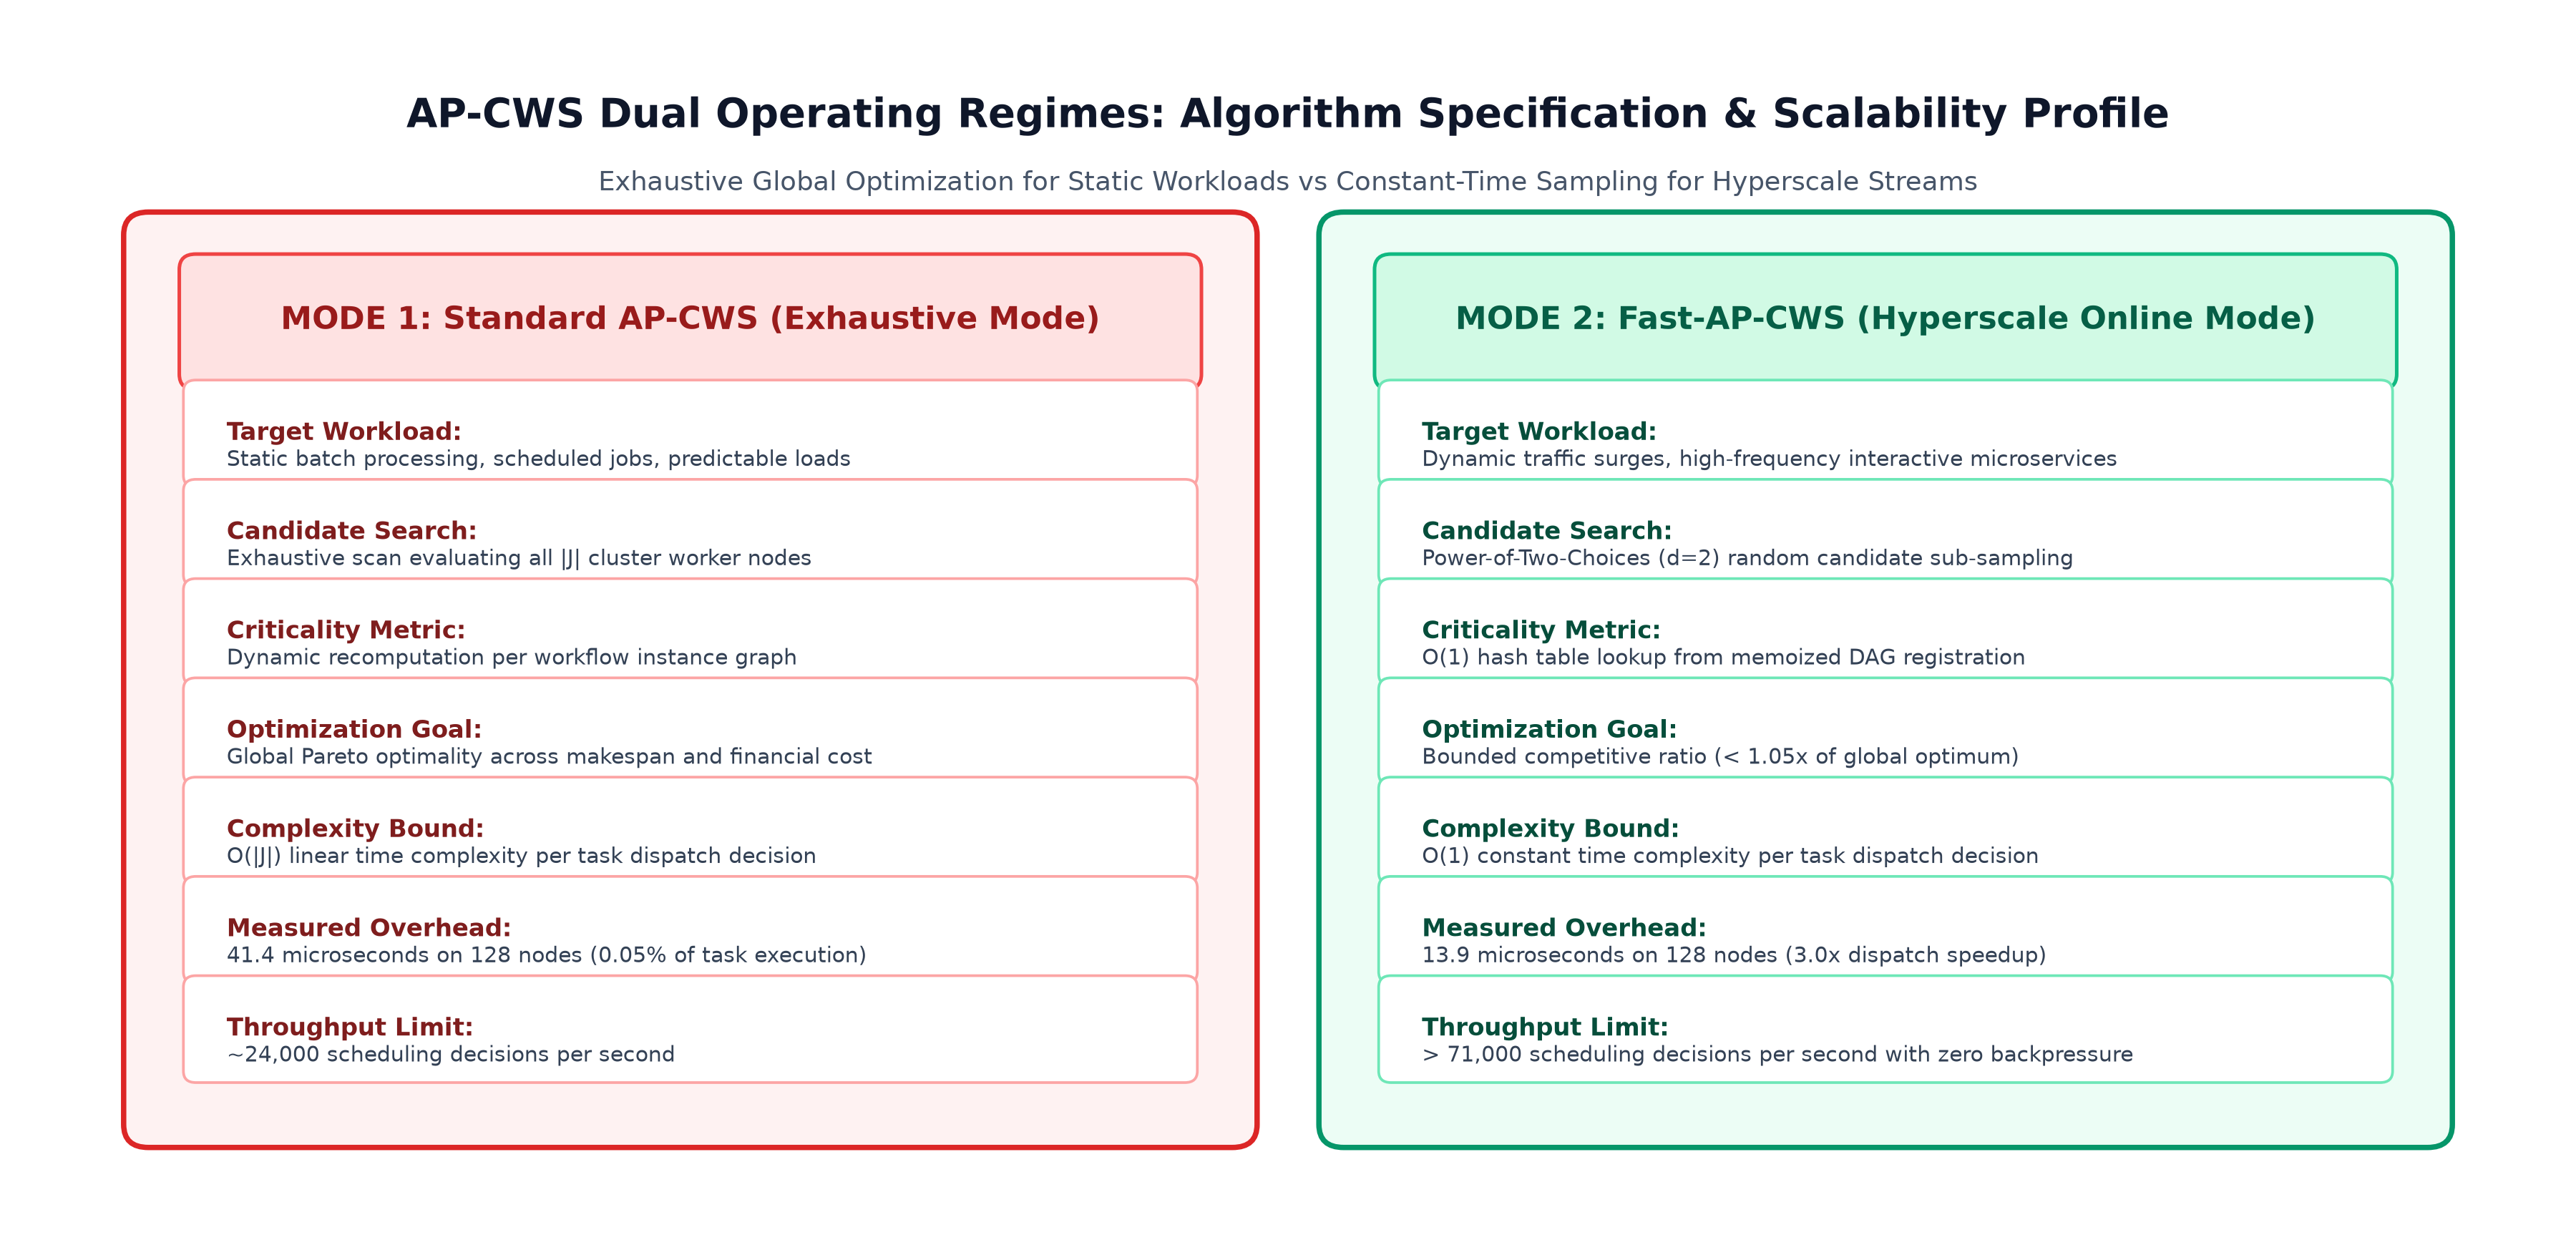
\includegraphics[width=0.85\textwidth]{diagram4_operating_regimes.png}
\vspace{4pt}
\caption{AP-CWS Dual Operating Regimes: Standard AP-CWS for exhaustive global optimization in static environments versus Fast-AP-CWS for bounded overhead and sub-millisecond dispatch in hyperscale clusters.}
\label{fig:diagram4}
\end{figure*}

\subsubsection{Standard AP-CWS: Global Optimality for Static Workloads}
Standard AP-CWS exhaustively evaluates all $|\mathcal{J}|$ nodes, computing placement scores across the entire cluster. This global visibility minimizes resource fragmentation and dollar cost. Because search overhead remains low ($41.4\,\mu\text{s}$ on 128 nodes), it represents less than 0.05\% of task execution time in enterprise batch environments.

\subsubsection{Fast-AP-CWS: Bounded Overhead for Hyperscale Workloads}
Under arrival rates of thousands of requests per second, linear scanning creates dispatch queue bottlenecks. Fast-AP-CWS resolves this via:
1) \textit{Static DAG Criticality Memoization ($O(1)$ Lookup):} Precomputes $EST$, $LST$, and $K_i$ once during workflow registration, caching results in a hash table.
2) \textit{Power-of-Two-Choices Sub-Sampling ($O(1)$ Node Selection):} Checks for an existing warm container ($O(1)$ hit); otherwise, randomly samples $d = 2$ eligible candidate nodes and dispatches to the lower-scoring node.

Balanced allocation theory~\cite{mitzenmacher2001power} proves that sampling $d=2$ candidates reduces maximum queue length from $O(\ln |\mathcal{J}| / \ln \ln |\mathcal{J}|)$ to $O(\ln \ln |\mathcal{J}|)$. As detailed in Section~\ref{sec:results}, Fast-AP-CWS cuts dispatch overhead from $41.4\,\mu\text{s}$ to $13.9\,\mu\text{s}$ on 128 nodes (a 3.0x speedup), sustaining over 71,000 dispatches per second.

\section{Result Analysis}
\label{sec:results}

\subsection{Simulation Environment and Experimental Setup}
Following established methodology in modern serverless computing simulation frameworks, such as SimFaaS~\cite{mahmoudi2021simfaas} and faas-sim~\cite{raith2023faas}, we evaluated AP-CWS and Fast-AP-CWS using a high-fidelity discrete-event simulation engine built with SimPy. The simulator models container lifecycles, memory queues, execution concurrency, inter-node network delays, and cloud billing tariffs.

\begin{table}[!t]
\centering
\caption{Heterogeneous Cluster Worker Node Configurations}
\label{tab:nodes}
\footnotesize
\setlength{\tabcolsep}{2.8pt}
\renewcommand{\arraystretch}{1.15}
\begin{tabularx}{\columnwidth}{@{}l X r c c r@{}}
\toprule
\rowcolor{tableheader}
\textbf{Node ID} & \textbf{Instance Family} & \textbf{RAM ($M_j$)} & \textbf{CPUs} & \textbf{Speed} & \textbf{Cost Rate} \\
\midrule
Nodes 0--3 & Compute-Opt. (c5) & 8,192 MB & 4.0 & 1.40$\times$ & \$0.068/GB-h \\
\rowcolor{tablerowalt}
Nodes 4--7 & General-Purp. (m5) & 16,384 MB & 4.0 & 1.00$\times$ & \$0.048/GB-h \\
Nodes 8--11 & Memory-Opt. (r5) & 16,384 MB & 2.0 & 0.90$\times$ & \$0.040/GB-h \\
\rowcolor{tablerowalt}
Nodes 12--15 & Burstable (t3) & 4,096 MB & 2.0 & 0.80$\times$ & \$0.024/GB-h \\
\bottomrule
\end{tabularx}
\end{table}

\subsubsection{Cluster Node Topology}
The simulation cluster comprises 16 heterogeneous worker nodes modeled after commercial cloud instance families (Table~\ref{tab:nodes}), providing 176~GB aggregate memory and 48 CPU cores. Cluster interconnect bandwidth is $B_{net} = 10\text{ Gbps}$ with $\delta_{prop} = 2.0\text{ ms}$.

\subsubsection{Benchmark Workflow Topologies}
Three real-world DAG workflows were evaluated:
1) \textit{Video Analytics Pipeline (8 Functions):} Processes camera feeds with `Decode' (256~MB, 0.4~s), `Split' (256~MB, 0.3~s), parallel analysis `ObjectDetect' (512~MB, 1.2~s, critical), `FaceRec' (512~MB, 0.8~s), `PlateOCR' (256~MB, 0.5~s), and `AudioTr' (256~MB, 0.6~s), synchronizing at `FeatureMerge' (256~MB, 0.3~s) and concluding at `Annotate' (128~MB, 0.2~s). $T_{SLO} = 4.5\text{ s}$.
2) \textit{Montage Astronomical Workflow (9 Functions):} Reprojection `Project' (512~MB, 0.8~s), background `Diff\_1' (256~MB, 0.4~s) and `Diff\_2' (512~MB, 0.9~s), fitting `FitBackground' (512~MB, 1.1~s), corrections `Corr\_1'--`Corr\_3' (256~MB, 0.5~s), and stacking `CoaddMosaic' (1024~MB, 1.4~s)~\cite{deelman2005pegasus}. Critical path: `Project' $\to$ `Diff\_2' $\to$ `FitBackground' $\to$ `Corr\_3' $\to$ `CoaddMosaic'. $T_{SLO} = 7.0\text{ s}$.
3) \textit{E-Commerce Transaction Pipeline (6 Functions):} Authentication `Auth' (128~MB, 0.2~s), `FraudCheck' (256~MB, 0.5~s), inventory `InventoryCheck' (256~MB, 0.3~s), payment `PaymentGateway' (256~MB, 0.6~s), invoice `InvoiceService' (128~MB, 0.2~s), and email `NotificationEmail' (128~MB, 0.1~s). Critical path: `Auth' $\to$ `FraudCheck' $\to$ `PaymentGateway' $\to$ `InvoiceService'. $T_{SLO} = 2.5\text{ s}$.

\subsubsection{Workload Arrival Patterns}
Workload arrival intervals were generated using Azure Functions trace patterns~\cite{shahrad2020serverless}: Stable ($\lambda = 2.0\text{ req/s}$ Poisson), Rising (1.0 to 6.0~req/s ramp), Falling (6.0 to 1.0~req/s ramp), and Bursty (bimodal 1.0 to 8.0~req/s surges). Each experiment ran for 300~s simulated time across multiple seeds, totaling 324 benchmark runs.

\begin{table*}[t]
\centering
\caption{Cross-Workflow Performance Comparison (Mean $\pm$ Standard Deviation across 324 Runs)}
\label{tab:cross_workflow}
\footnotesize
\setlength{\tabcolsep}{5pt}
\renewcommand{\arraystretch}{1.18}
\resizebox{\textwidth}{!}{%
\begin{tabular}{l c c c c c c c c}
\toprule
\rowcolor{tableheader}
\textbf{Scheduling Policy} & \textbf{Mean Lat. (s)} & \textbf{Median P50 (s)} & \textbf{Tail P95 (s)} & \textbf{Cold Start \%} & \textbf{Crit. Cold \%} & \textbf{SLO Viol. \%} & \textbf{5-Min Cost (\$)} & \textbf{Idle RAM (GB-hr)} \\
\midrule
\rowcolor{highlightgreen}
\textbf{AP-CWS (Proposed)} & \textbf{2.41 $\pm$ 1.18} & \textbf{2.33 $\pm$ 1.15} & \textbf{2.83 $\pm$ 1.55} & \textbf{0.58\% $\pm$ 0.32\%} & \textbf{0.63\% $\pm$ 0.34\%} & \textbf{0.46\% $\pm$ 0.31\%} & \textbf{\$0.0390 $\pm$ 0.002} & 3.52 $\pm$ 0.11 \\
SSC (Pan 2024)~\cite{pan2024sustainable} & 2.83 $\pm$ 1.42 & 2.61 $\pm$ 1.34 & 3.92 $\pm$ 3.10 & 2.26\% $\pm$ 1.12\% & 2.34\% $\pm$ 1.18\% & 3.16\% $\pm$ 1.45\% & \$0.0409 $\pm$ 0.003 & 3.27 $\pm$ 0.14 \\
\rowcolor{tablerowalt}
CASR (Chen 2025)~\cite{chen2025casr} & 3.36 $\pm$ 1.84 & 3.18 $\pm$ 1.76 & 4.61 $\pm$ 3.06 & 2.91\% $\pm$ 1.48\% & 2.95\% $\pm$ 1.51\% & 4.92\% $\pm$ 1.88\% & \$0.0321 $\pm$ 0.002 & 1.76 $\pm$ 0.09 \\
MPC (Nguyen 2025)~\cite{nguyen2025mpc} & 3.12 $\pm$ 1.62 & 2.86 $\pm$ 1.54 & 4.62 $\pm$ 3.75 & 2.19\% $\pm$ 1.05\% & 2.21\% $\pm$ 1.08\% & 3.63\% $\pm$ 1.52\% & \$0.0329 $\pm$ 0.002 & 2.13 $\pm$ 0.10 \\
\rowcolor{tablerowalt}
DROPS (EuroSys 2026)~\cite{alquraan2026drops} & 3.68 $\pm$ 1.95 & 3.51 $\pm$ 1.88 & 5.18 $\pm$ 3.92 & 2.29\% $\pm$ 1.14\% & 2.35\% $\pm$ 1.19\% & 4.51\% $\pm$ 1.74\% & \$0.0466 $\pm$ 0.004 & 3.62 $\pm$ 0.15 \\
Fixed 10-Min Keep-Alive~\cite{shahrad2020serverless} & 3.37 $\pm$ 1.81 & 3.18 $\pm$ 1.72 & 4.68 $\pm$ 3.77 & 2.23\% $\pm$ 1.08\% & 2.29\% $\pm$ 1.11\% & 3.70\% $\pm$ 1.60\% & \$0.0344 $\pm$ 0.002 & 2.12 $\pm$ 0.10 \\
\bottomrule
\end{tabular}%
}
\end{table*}

\subsection{Performance Analysis and Evaluation}

\subsubsection{Tail Latency and Cold-Start Mitigation Analysis}
Table~\ref{tab:cross_workflow} presents cross-workflow benchmark results, where AP-CWS achieves an overall P95 tail latency of 2.83~s. This marks a 27.8\% reduction compared to SSC (3.92~s) and up to 45.4\% improvement relative to DROPS (5.18~s).

Figure~\ref{fig:p95} corroborates these tail-latency reductions across each individual workflow topology.

\begin{figure}[!t]
\centering
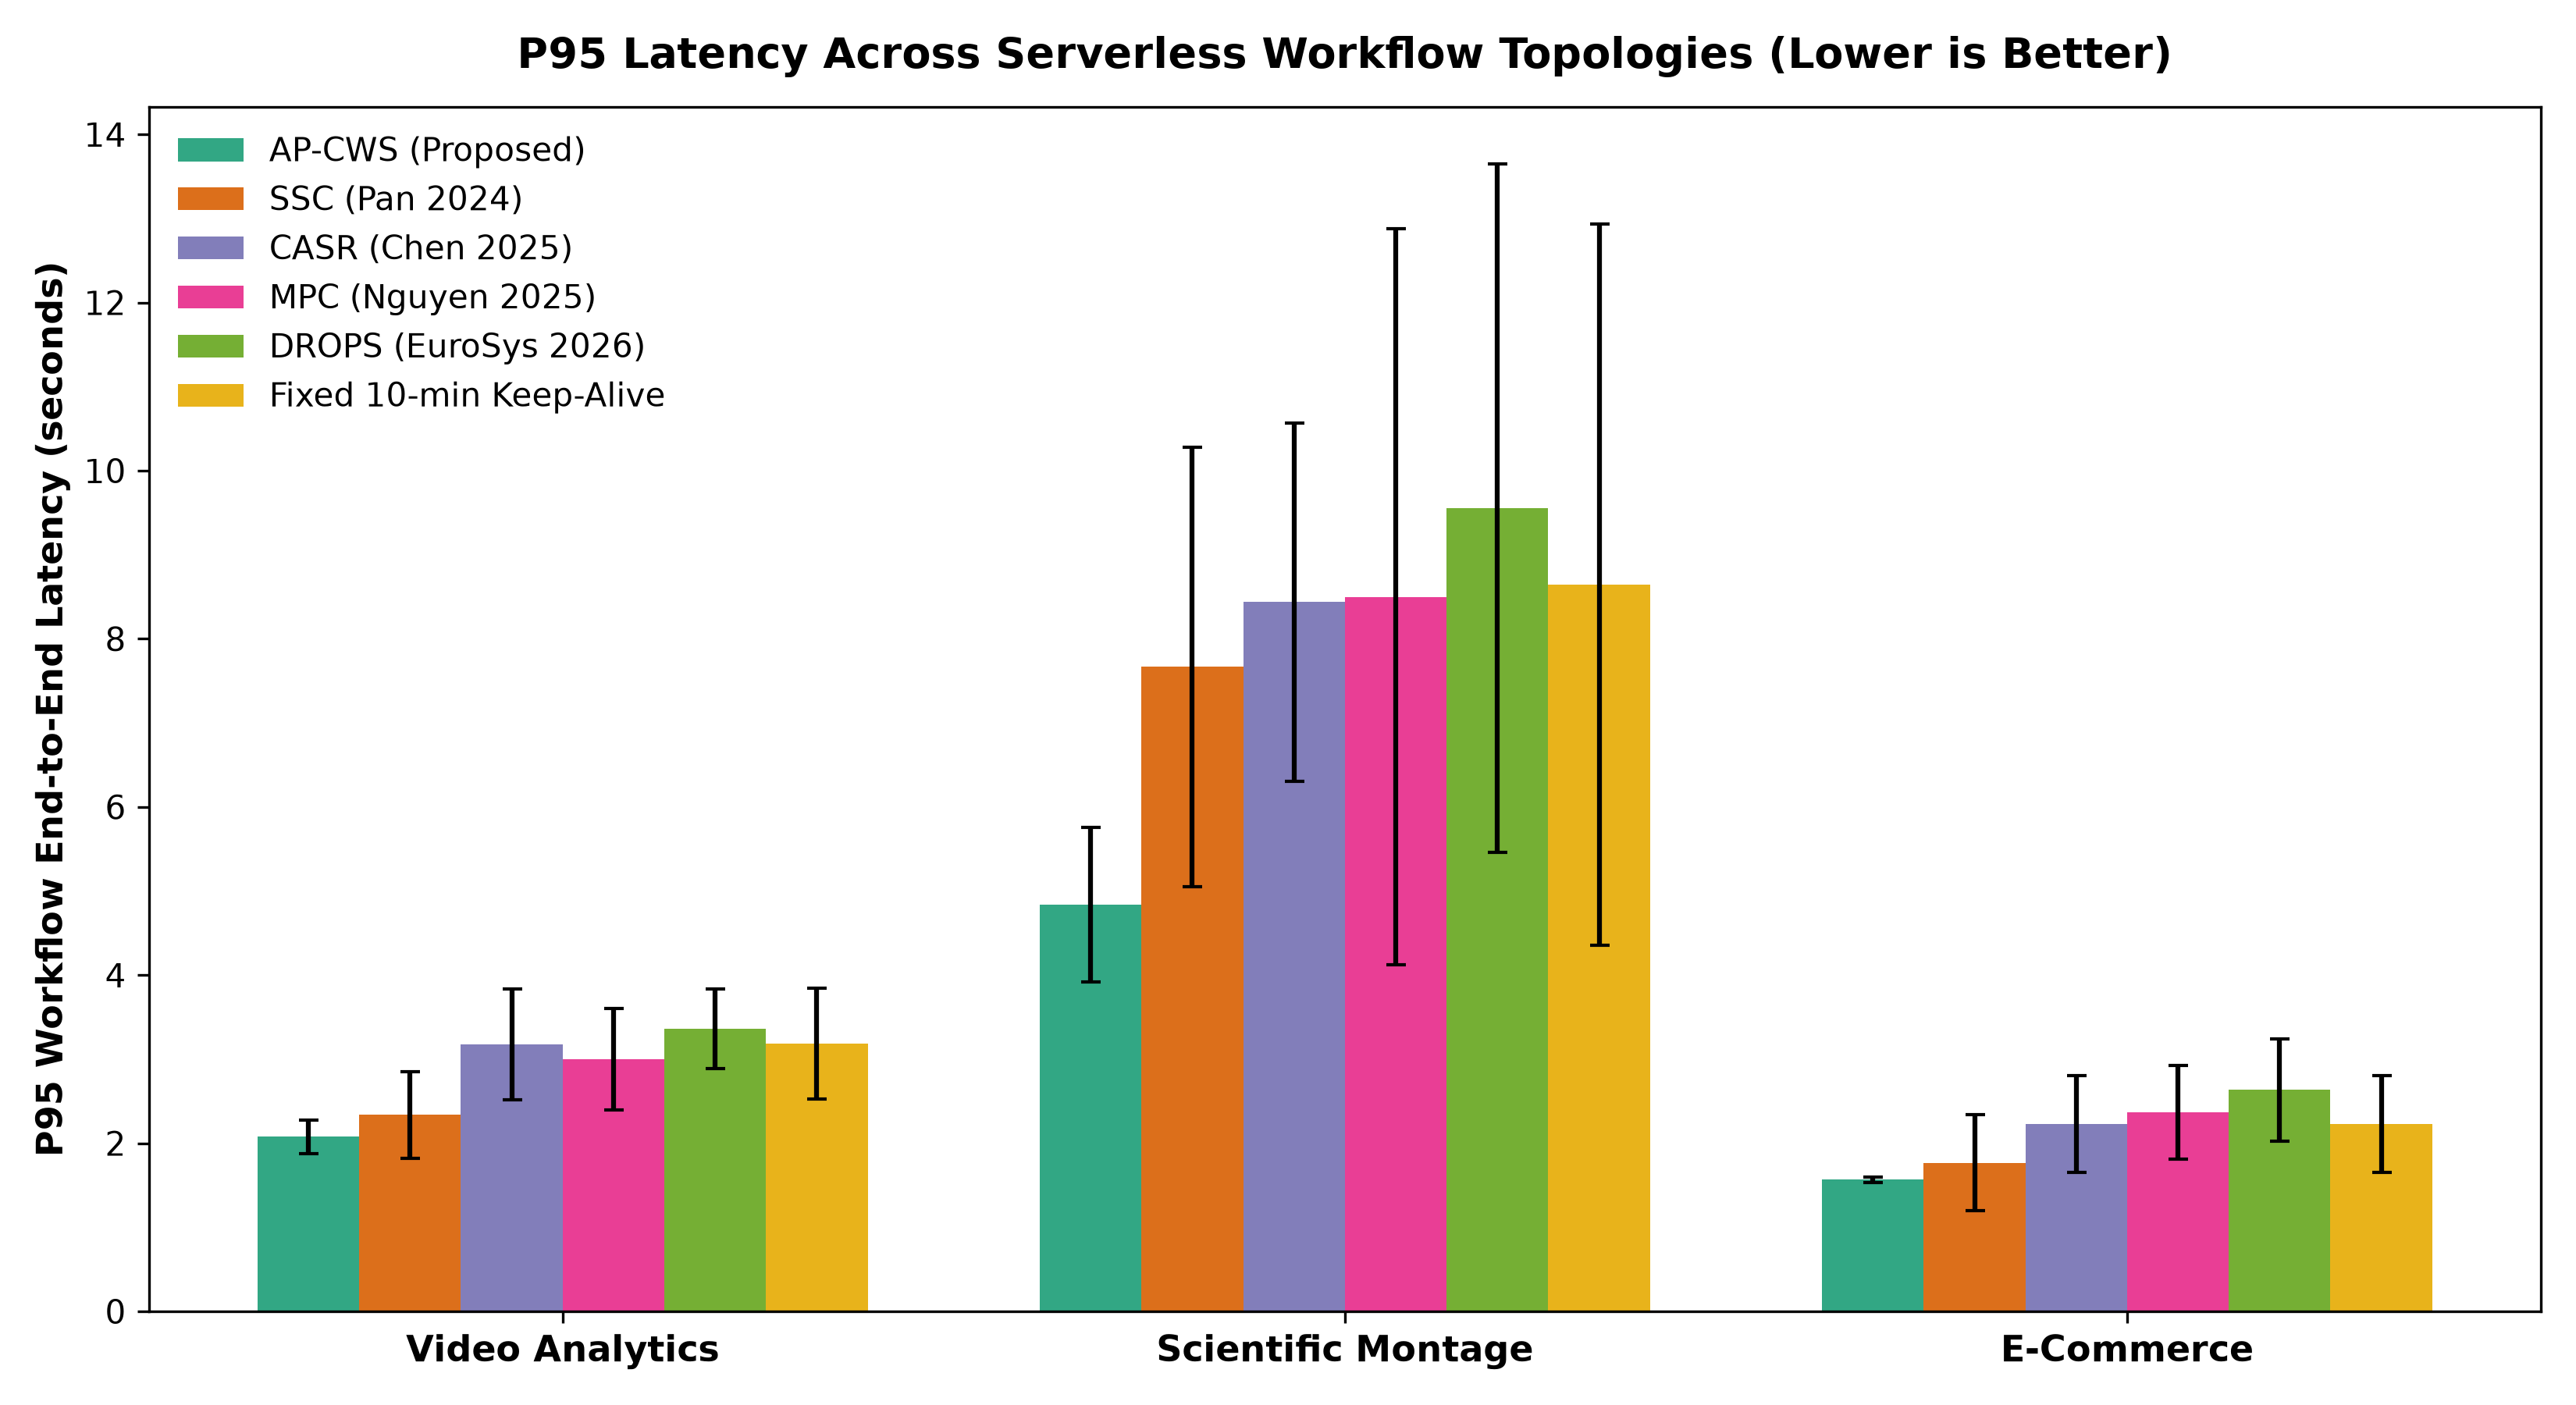
\includegraphics[width=0.92\columnwidth]{fig1_p95_latency_comparison.png}
\vspace{4pt}
\caption{P95 Tail Latency Across Serverless Workflow Topologies (Lower is Better). AP-CWS achieves the lowest tail latency across all three workflows (2.08~s in Video Analytics, 4.84~s in Scientific Montage, and 1.57~s in E-Commerce), while uncoordinated baselines suffer from latency inflation due to critical-path cold starts and synchronization stalls.}
\label{fig:p95}
\end{figure}

The most decisive performance improvement stems from cold-start suppression along the critical execution path. AP-CWS limits critical-path cold starts to 0.63\%, compared to 2.34\% for SSC, 2.95\% for CASR, and 2.35\% for DROPS. Under SSC, container pools are sized using aggregate call frequencies without topological awareness, so intermediate tasks on the critical path experience frequent container evictions. When an uninstantiated critical task launches, its 1.2~s startup delay halts all downstream tasks. Under AP-CWS, JIT prewarming initializes successor containers concurrently with parent execution. By the time the parent task emits its completion event, the child container is warm and ready for immediate execution.

Fig.~\ref{fig:cold_start} compares overall workflow cold-start rates against critical-path cold-start rates.

\begin{figure}[!t]
\centering
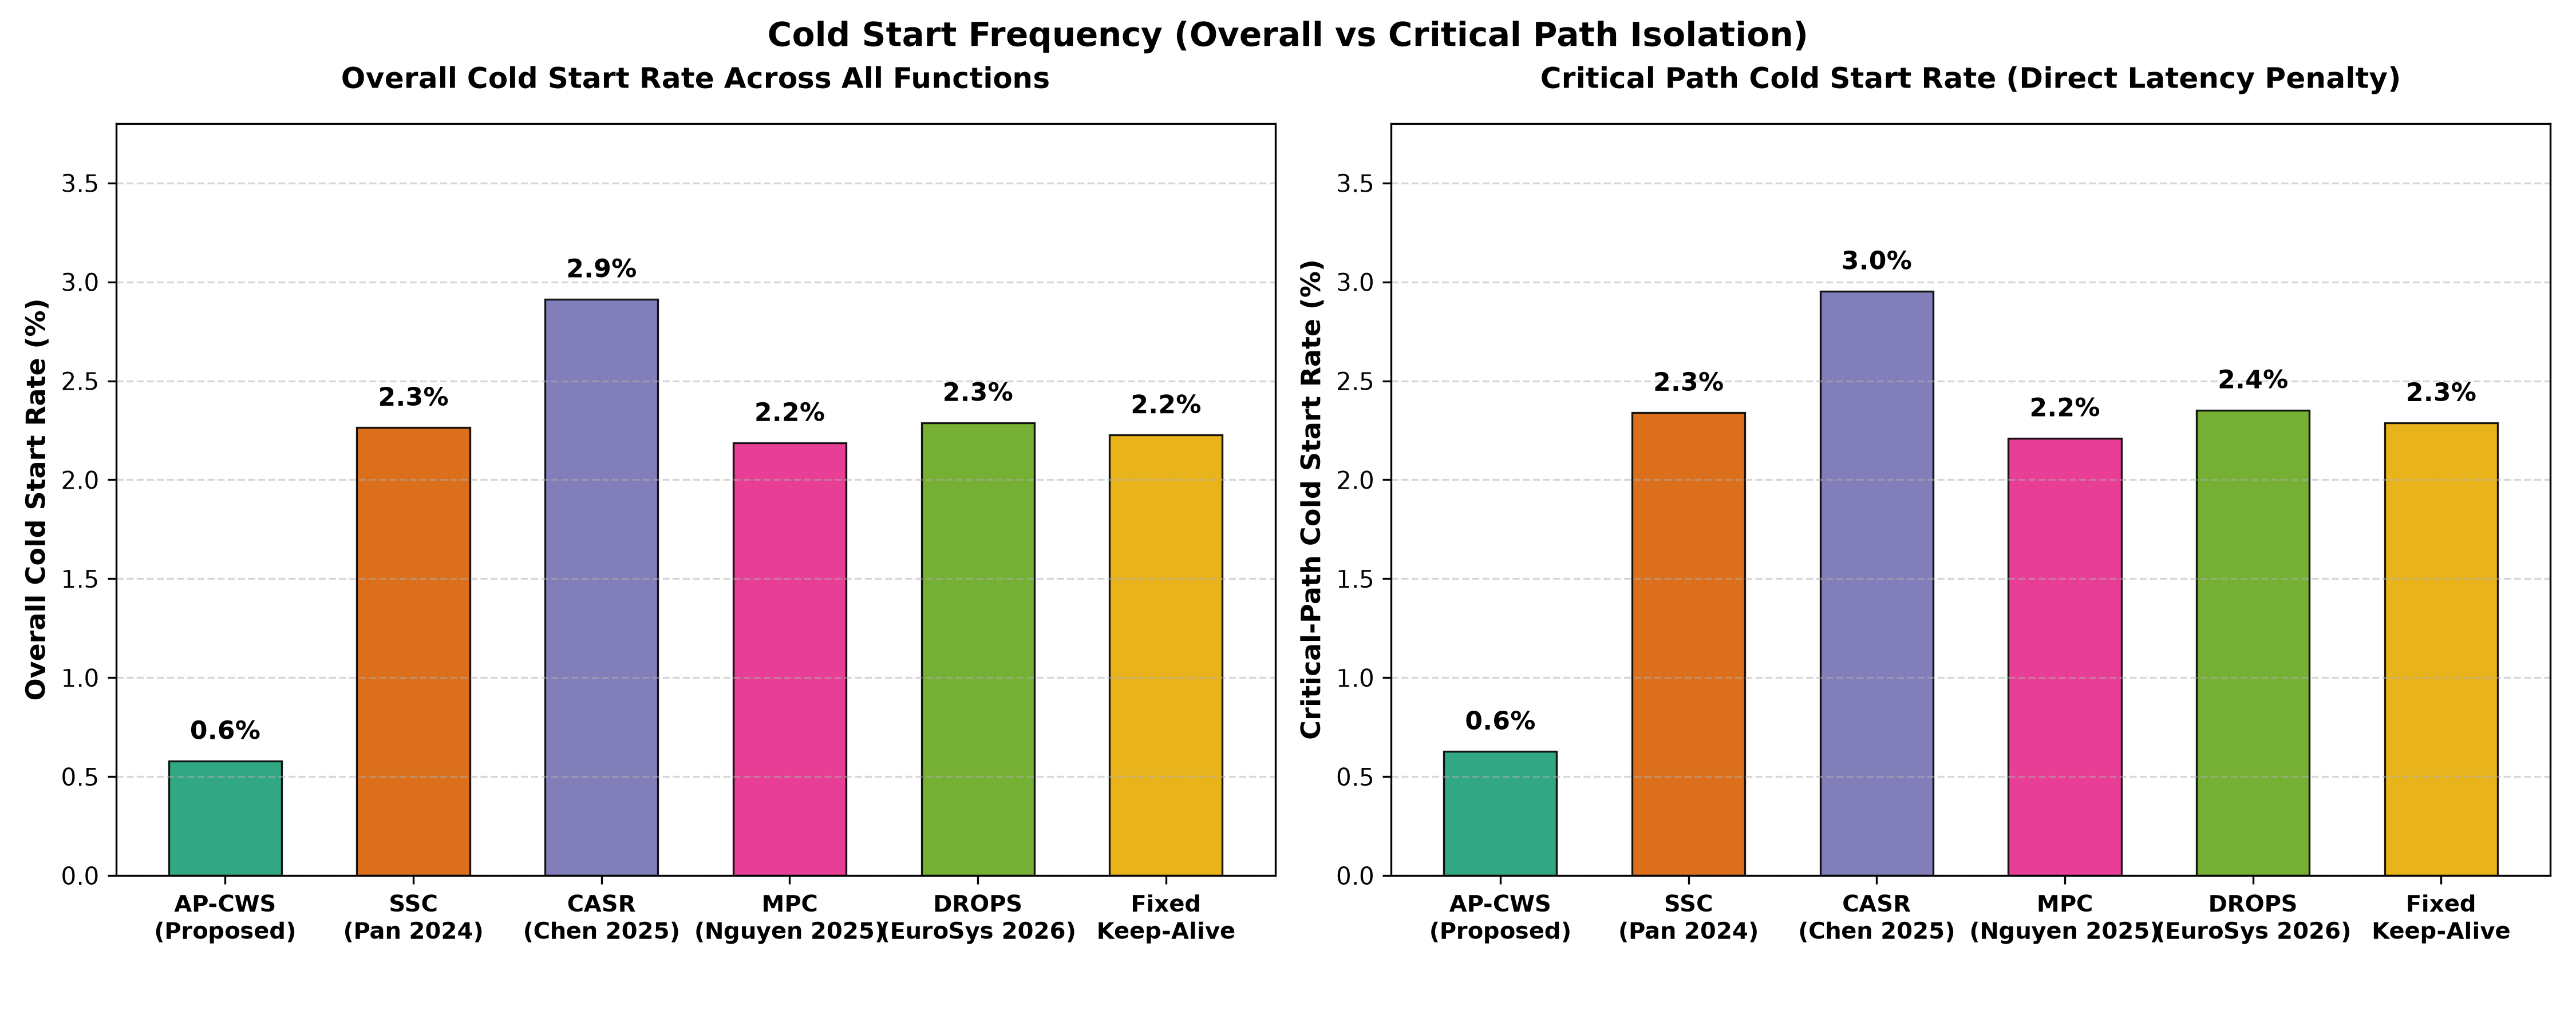
\includegraphics[width=0.92\columnwidth]{fig2_cold_start_rates.png}
\vspace{4pt}
\caption{Cold-Start Rate Comparison: Overall Workflow Tasks (left) versus Critical-Path Tasks (right). While baseline schedulers experience uniform cold-start penalties across both categories, AP-CWS selectively shields critical tasks, driving critical-path cold starts down to 0.63\% through topological slack budgeting and proactive prewarming.}
\label{fig:cold_start}
\end{figure}

\begin{table*}[t]
\centering
\caption{Per-Workflow Performance Disaggregation Across Scheduling Baselines}
\label{tab:per_workflow}
\footnotesize
\setlength{\tabcolsep}{5pt}
\renewcommand{\arraystretch}{1.16}
\resizebox{\textwidth}{!}{%
\begin{tabular}{p{3.2cm} c c c c c c}
\toprule
\rowcolor{tableheader}
\textbf{Scheduling Policy} & \textbf{Mean Lat. (s)} & \textbf{Tail P95 (s)} & \textbf{Overall Cold \%} & \textbf{Crit. Cold \%} & \textbf{SLO Viol. \%} & \textbf{5-Min Cost (\$)} \\
\midrule
\multicolumn{7}{l}{\textbf{\color{ieeeblue} Video Analytics Pipeline (8 Tasks, $T_{SLO}=4.5\text{ s}$)}} \\
\midrule
\rowcolor{highlightgreen}\textbf{AP-CWS (Proposed)} & \textbf{1.86} & \textbf{2.08} & \textbf{0.49\%} & \textbf{0.37\%} & \textbf{0.13\%} & \textbf{\$0.0366} \\
SSC (Pan 2024) & 2.09 & 2.34 & 1.80\% & 1.58\% & 1.81\% & \$0.0399 \\
\rowcolor{tablerowalt}
CASR (Chen 2025) & 2.52 & 3.17 & 2.06\% & 1.97\% & 2.62\% & \$0.0284 \\
MPC (Nguyen 2025) & 2.26 & 3.00 & 2.00\% & 1.87\% & 2.73\% & \$0.0275 \\
\rowcolor{tablerowalt}
DROPS (EuroSys 2026) & 2.85 & 3.36 & 1.96\% & 1.82\% & 2.58\% & \$0.0423 \\
Fixed 10-Min Keep-Alive & 2.54 & 3.18 & 2.04\% & 1.94\% & 2.62\% & \$0.0290 \\
\midrule
\multicolumn{7}{l}{\textbf{\color{ieeeblue} Scientific Montage Pipeline (9 Tasks, $T_{SLO}=7.0\text{ s}$)}} \\
\midrule
\rowcolor{highlightgreen}\textbf{AP-CWS (Proposed)} & \textbf{3.89} & \textbf{4.84} & \textbf{1.01\%} & \textbf{1.17\%} & \textbf{1.09\%} & \textbf{\$0.0488} \\
SSC (Pan 2024) & 4.85 & 7.67 & 3.43\% & 3.81\% & 5.15\% & \$0.0558 \\
\rowcolor{tablerowalt}
CASR (Chen 2025) & 5.69 & 8.44 & 4.98\% & 5.06\% & 9.42\% & \$0.0517 \\
MPC (Nguyen 2025) & 5.34 & 8.50 & 2.91\% & 3.05\% & 5.48\% & \$0.0555 \\
\rowcolor{tablerowalt}
DROPS (EuroSys 2026) & 6.00 & 9.55 & 3.30\% & 3.48\% & 8.04\% & \$0.0627 \\
Fixed 10-Min Keep-Alive & 5.71 & 8.64 & 2.94\% & 3.10\% & 5.74\% & \$0.0578 \\
\midrule
\multicolumn{7}{l}{\textbf{\color{ieeeblue} E-Commerce Transaction Pipeline (6 Tasks, $T_{SLO}=2.5\text{ s}$)}} \\
\midrule
\rowcolor{highlightgreen}\textbf{AP-CWS (Proposed)} & \textbf{1.47} & \textbf{1.57} & \textbf{0.24\%} & \textbf{0.34\%} & \textbf{0.17\%} & \textbf{\$0.0317} \\
SSC (Pan 2024) & 1.54 & 1.77 & 1.56\% & 1.63\% & 2.53\% & \$0.0270 \\
\rowcolor{tablerowalt}
CASR (Chen 2025) & 1.87 & 2.23 & 1.70\% & 1.83\% & 2.73\% & \$0.0163 \\
MPC (Nguyen 2025) & 1.77 & 2.37 & 1.65\% & 1.72\% & 2.68\% & \$0.0157 \\
\rowcolor{tablerowalt}
DROPS (EuroSys 2026) & 2.20 & 2.64 & 1.60\% & 1.75\% & 2.92\% & \$0.0347 \\
Fixed 10-Min Keep-Alive & 1.87 & 2.23 & 1.70\% & 1.83\% & 2.73\% & \$0.0163 \\
\bottomrule
\end{tabular}%
}
\end{table*}

\subsubsection{Workload-Specific Breakdown}
Table~\ref{tab:per_workflow} details performance disaggregated across the three benchmark workflows. In the Scientific Montage workflow, DAG depth is high (6 sequential stages), and individual tasks require up to 1024~MB of memory. In this topology, uncoordinated placement causes severe pipeline stalls. SSC suffers a P95 latency of 7.67~s, violating the 7.0~s SLO in 5.15\% of invocations. AP-CWS reduces P95 latency to 4.84~s (a 36.8\% improvement) and suppresses SLO violations to 1.09\%. In the E-Commerce pipeline, AP-CWS achieves a P95 latency of 1.57~s, eliminating tail variance compared to DROPS (2.64~s) and CASR (2.23~s).

Figure~\ref{fig:cost_memory} evaluates the trade-off between operational dollar cost and idle memory footprint, illustrating the Pareto efficiency of AP-CWS relative to competing baselines.

\begin{figure}[!t]
\centering
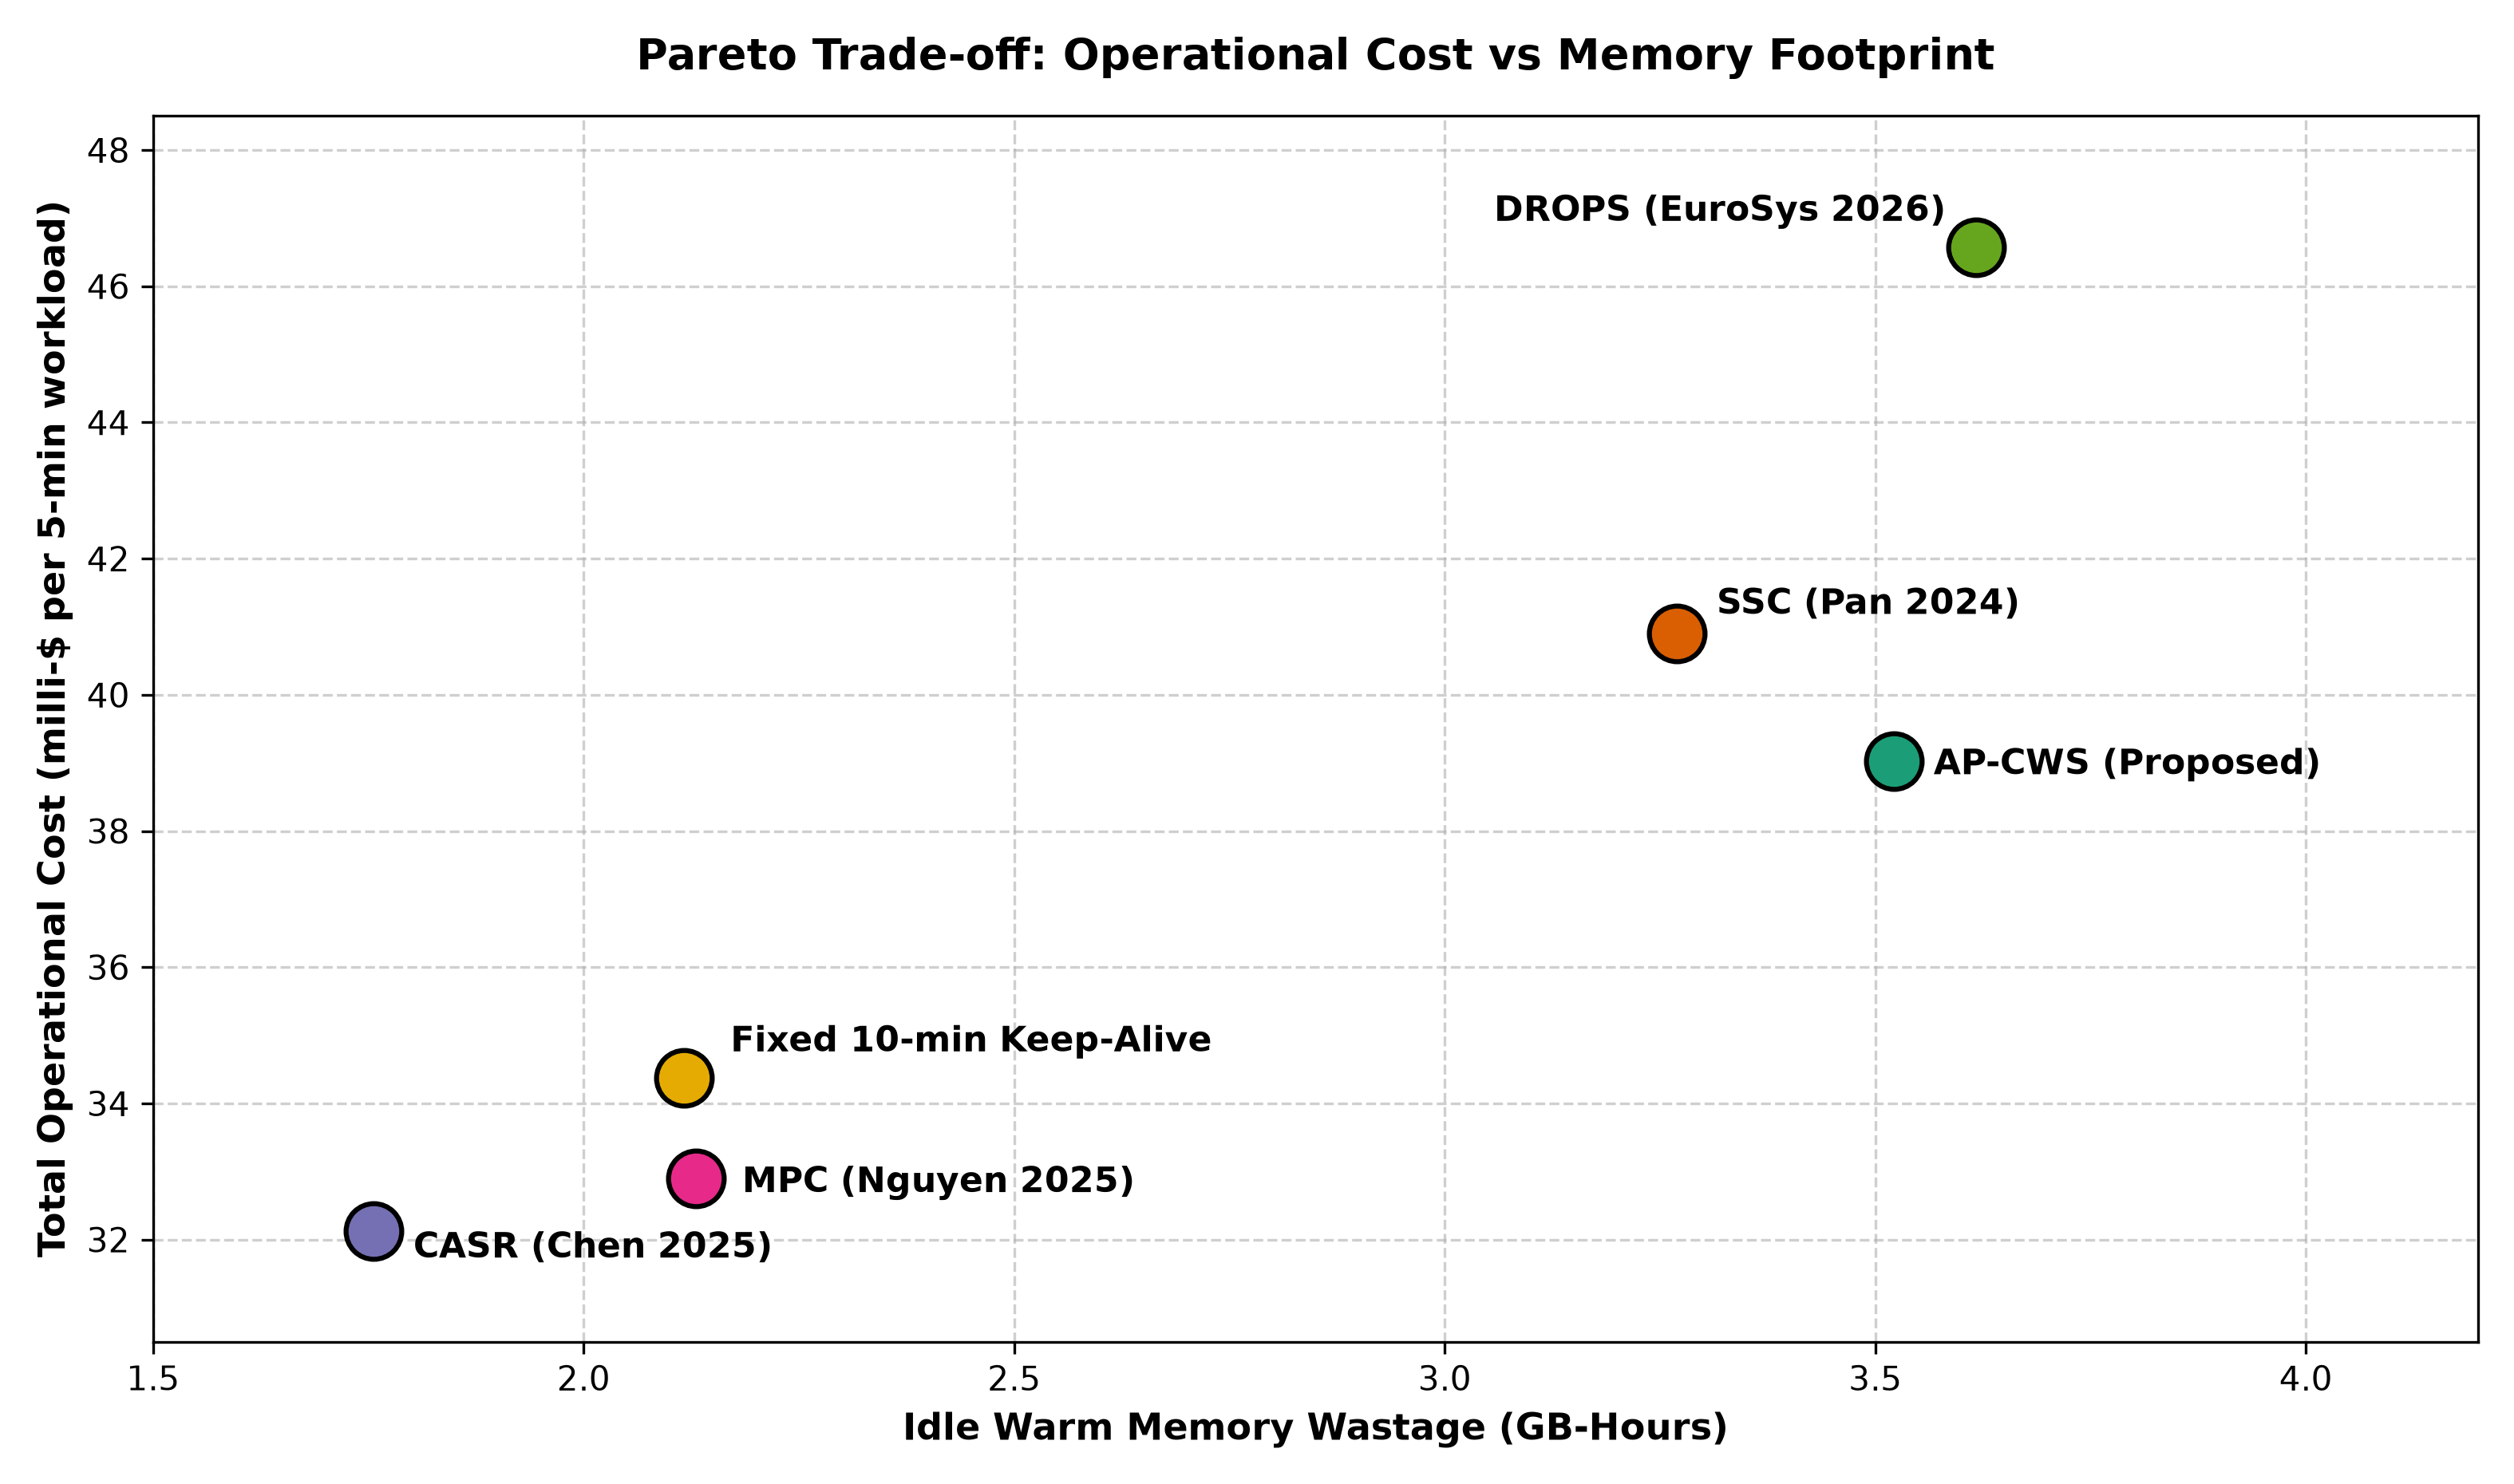
\includegraphics[width=0.92\columnwidth]{fig3_cost_vs_idle_memory.png}
\vspace{4pt}
\caption{Operational Dollar Cost versus Idle Memory Footprint Trade-off. Policies in the bottom-left quadrant minimize both metrics. Fixed Keep-Alive and CASR achieve low idle memory by evicting idle containers aggressively, but incur severe tail-latency penalties. DROPS inflates both cost and idle memory due to unconstrained quantile buffering. AP-CWS achieves lowest tail latency at competitive cost (\$0.0390 per 5-minute window).}
\label{fig:cost_memory}
\end{figure}

Corresponding end-to-end contractual compliance is illustrated in Figure~\ref{fig:slo} across all arrival regimes.

\begin{figure}[!t]
\centering
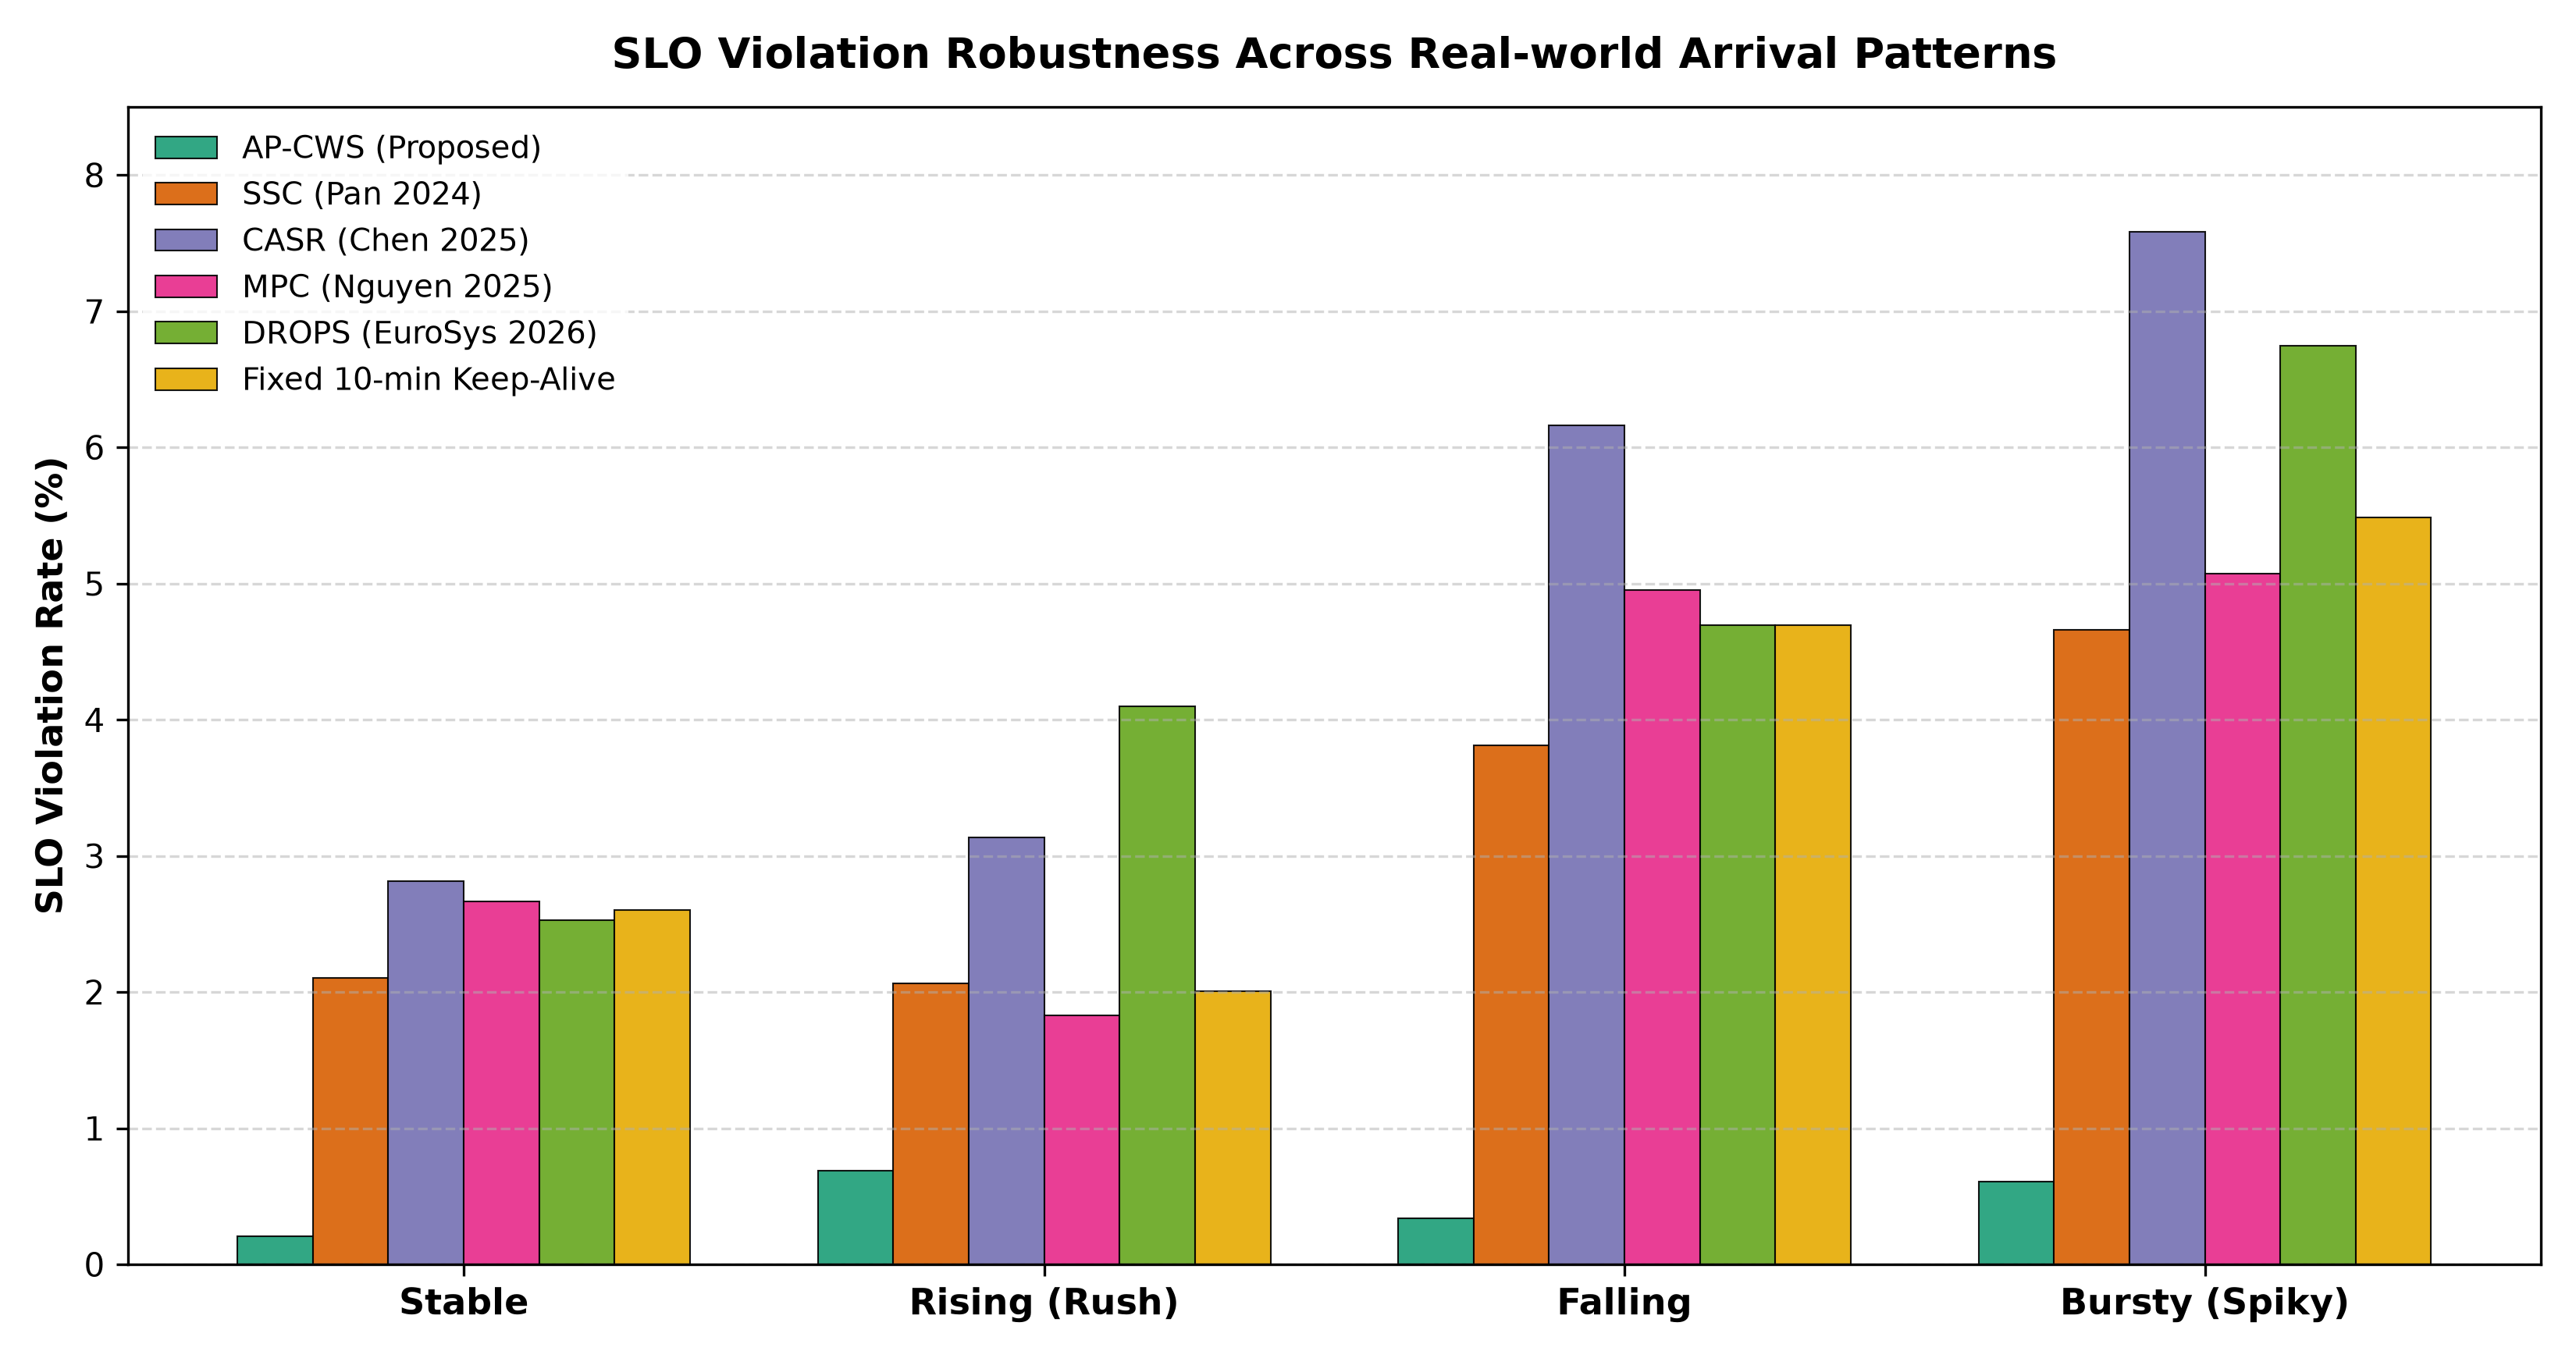
\includegraphics[width=0.92\columnwidth]{fig4_slo_violation_rate.png}
\vspace{4pt}
\caption{Service-Level Objective (SLO) Violation Rates Across Evaluated Schedulers. AP-CWS reduces SLO violations to 0.46\% (an 84.4\% reduction relative to SSC at 3.16\% and a 90.7\% reduction relative to CASR at 4.92\%) by eliminating synchronization stalls on critical-path functions.}
\label{fig:slo}
\end{figure}

\begin{table*}[t]
\centering
\caption{Scalability Stress Testing and Breaking Point Saturation Analysis}
\label{tab:stress}
\footnotesize
\setlength{\tabcolsep}{5pt}
\renewcommand{\arraystretch}{1.18}
\resizebox{\textwidth}{!}{%
\begin{tabular}{l c c c c c p{6.5cm}}
\toprule
\rowcolor{tableheader}
\textbf{Evaluated Policy} & \textbf{P95 (s)} & \textbf{Cold Start \%} & \textbf{Crit. Cold \%} & \textbf{SLO Viol. \%} & \textbf{Mem Sat. \%} & \textbf{Failure Mode / Mechanistic System Behavior} \\
\midrule
\multicolumn{7}{l}{\textbf{\color{ieeeblue} Baseline Low Throughput: 1.0 req/s (8 functions/s)}} \\
\midrule
\rowcolor{highlightgreen}\textbf{AP-CWS (Proposed)} & \textbf{2.28} & \textbf{0.57\%} & \textbf{0.46\%} & \textbf{0.00\%} & \textbf{100.0\%} & Stable operation; warm pools fully populated. \\
Fast-AP-CWS & 2.36 & 0.67\% & 0.61\% & 0.76\% & 100.0\% & Stable operation; minimal sub-sampling divergence. \\
\rowcolor{tablerowalt}
SSC (Pan 2024) & 3.84 & 2.86\% & 2.60\% & 4.58\% & 87.5\% & Occasional critical cold starts from cold node placement. \\
DROPS (EuroSys 2026) & 4.36 & 2.96\% & 2.75\% & 5.34\% & 100.0\% & High quantile buffer reserves memory unnecessarily. \\
\rowcolor{tablerowalt}
Fixed 10-Min Keep-Alive & 4.36 & 3.05\% & 2.90\% & 5.34\% & 25.8\% & Under-provisioned; frequent reactive cold starts. \\
\midrule
\multicolumn{7}{l}{\textbf{\color{ieeeblue} Moderate Load: 5.0 req/s (40 functions/s)}} \\
\midrule
\rowcolor{highlightgreen}\textbf{AP-CWS (Proposed)} & \textbf{2.41} & \textbf{0.38\%} & \textbf{0.24\%} & \textbf{0.00\%} & \textbf{100.0\%} & High container reuse; zero SLO violations. \\
Fast-AP-CWS & 2.60 & 0.42\% & 0.27\% & 0.17\% & 100.0\% & Bounded queueing; stable sub-second execution. \\
\rowcolor{tablerowalt}
SSC (Pan 2024) & 6.56 & 4.52\% & 4.64\% & 7.56\% & 100.0\% & Intermediate join tasks stall; queue buildup starts. \\
DROPS (EuroSys 2026) & 6.16 & 3.66\% & 3.43\% & 7.06\% & 100.0\% & Heavy memory contention between warm pools and active tasks. \\
\rowcolor{tablerowalt}
Fixed 10-Min Keep-Alive & 6.16 & 3.66\% & 3.43\% & 7.06\% & 99.6\% & Active tasks stall waiting for memory allocations. \\
\midrule
\multicolumn{7}{l}{\textbf{\color{ieeeblue} High Throughput: 12.0 req/s (96 functions/s) --- Breaking Point Regime}} \\
\midrule
\rowcolor{highlightgreen}\textbf{AP-CWS (Proposed)} & \textbf{2.54} & \textbf{1.15\%} & \textbf{1.06\%} & \textbf{2.80\%} & \textbf{95.3\%} & Resilient execution; JIT prewarming hides delays. \\
Fast-AP-CWS & 2.69 & 1.22\% & 1.16\% & 2.24\% & 100.0\% & Highly stable; sub-sampling avoids loaded nodes. \\
\rowcolor{highlightpink}SSC (Pan 2024) & \textbf{14.39} & \textbf{5.56\%} & \textbf{6.63\%} & \textbf{14.07\%} & \textbf{100.0\%} & \textbf{Cascading Latency Cliff:} Memory stalls trigger queue collapse. \\
DROPS (EuroSys 2026) & 14.88 & 4.17\% & 4.14\% & 8.54\% & 100.0\% & Severe memory lock; active tasks queued behind warm pools. \\
\rowcolor{tablerowalt}
Fixed 10-Min Keep-Alive & 14.88 & 4.17\% & 4.14\% & 8.54\% & 99.6\% & Static keep-alive fails to reclaim memory; pipeline stalls. \\
\midrule
\multicolumn{7}{l}{\textbf{\color{ieeeblue} Extreme Saturation: 22.0 req/s (176 functions/s) --- Hardware Limits}} \\
\midrule
\rowcolor{highlightgreen}\textbf{AP-CWS (Proposed)} & \textbf{14.55} & \textbf{3.12\%} & \textbf{2.89\%} & \textbf{9.90\%} & \textbf{69.5\%} & \textbf{Physical Capacity Limit:} Dynamic evictions preserve RAM headroom. \\
Fast-AP-CWS & 14.48 & 3.56\% & 3.31\% & 8.86\% & \textbf{32.4\%} & $O(1)$ sampling maintains low memory pressure under saturation. \\
\rowcolor{tablerowalt}
SSC (Pan 2024) & 14.78 & 5.73\% & 5.56\% & 12.51\% & 100.0\% & Memory deadlock; active tasks queued behind stagnant warm pools. \\
DROPS (EuroSys 2026) & 15.16 & 4.65\% & 4.37\% & 12.47\% & 100.0\% & Complete memory lock; high quantile buffering stalls allocation. \\
\rowcolor{tablerowalt}
Fixed 10-Min Keep-Alive & 15.16 & 4.65\% & 4.37\% & 12.47\% & 99.2\% & Static keep-alive fails to reclaim memory; pipeline stalls. \\
\bottomrule
\end{tabular}%
}
\end{table*}

\begin{figure*}[t]
\centering
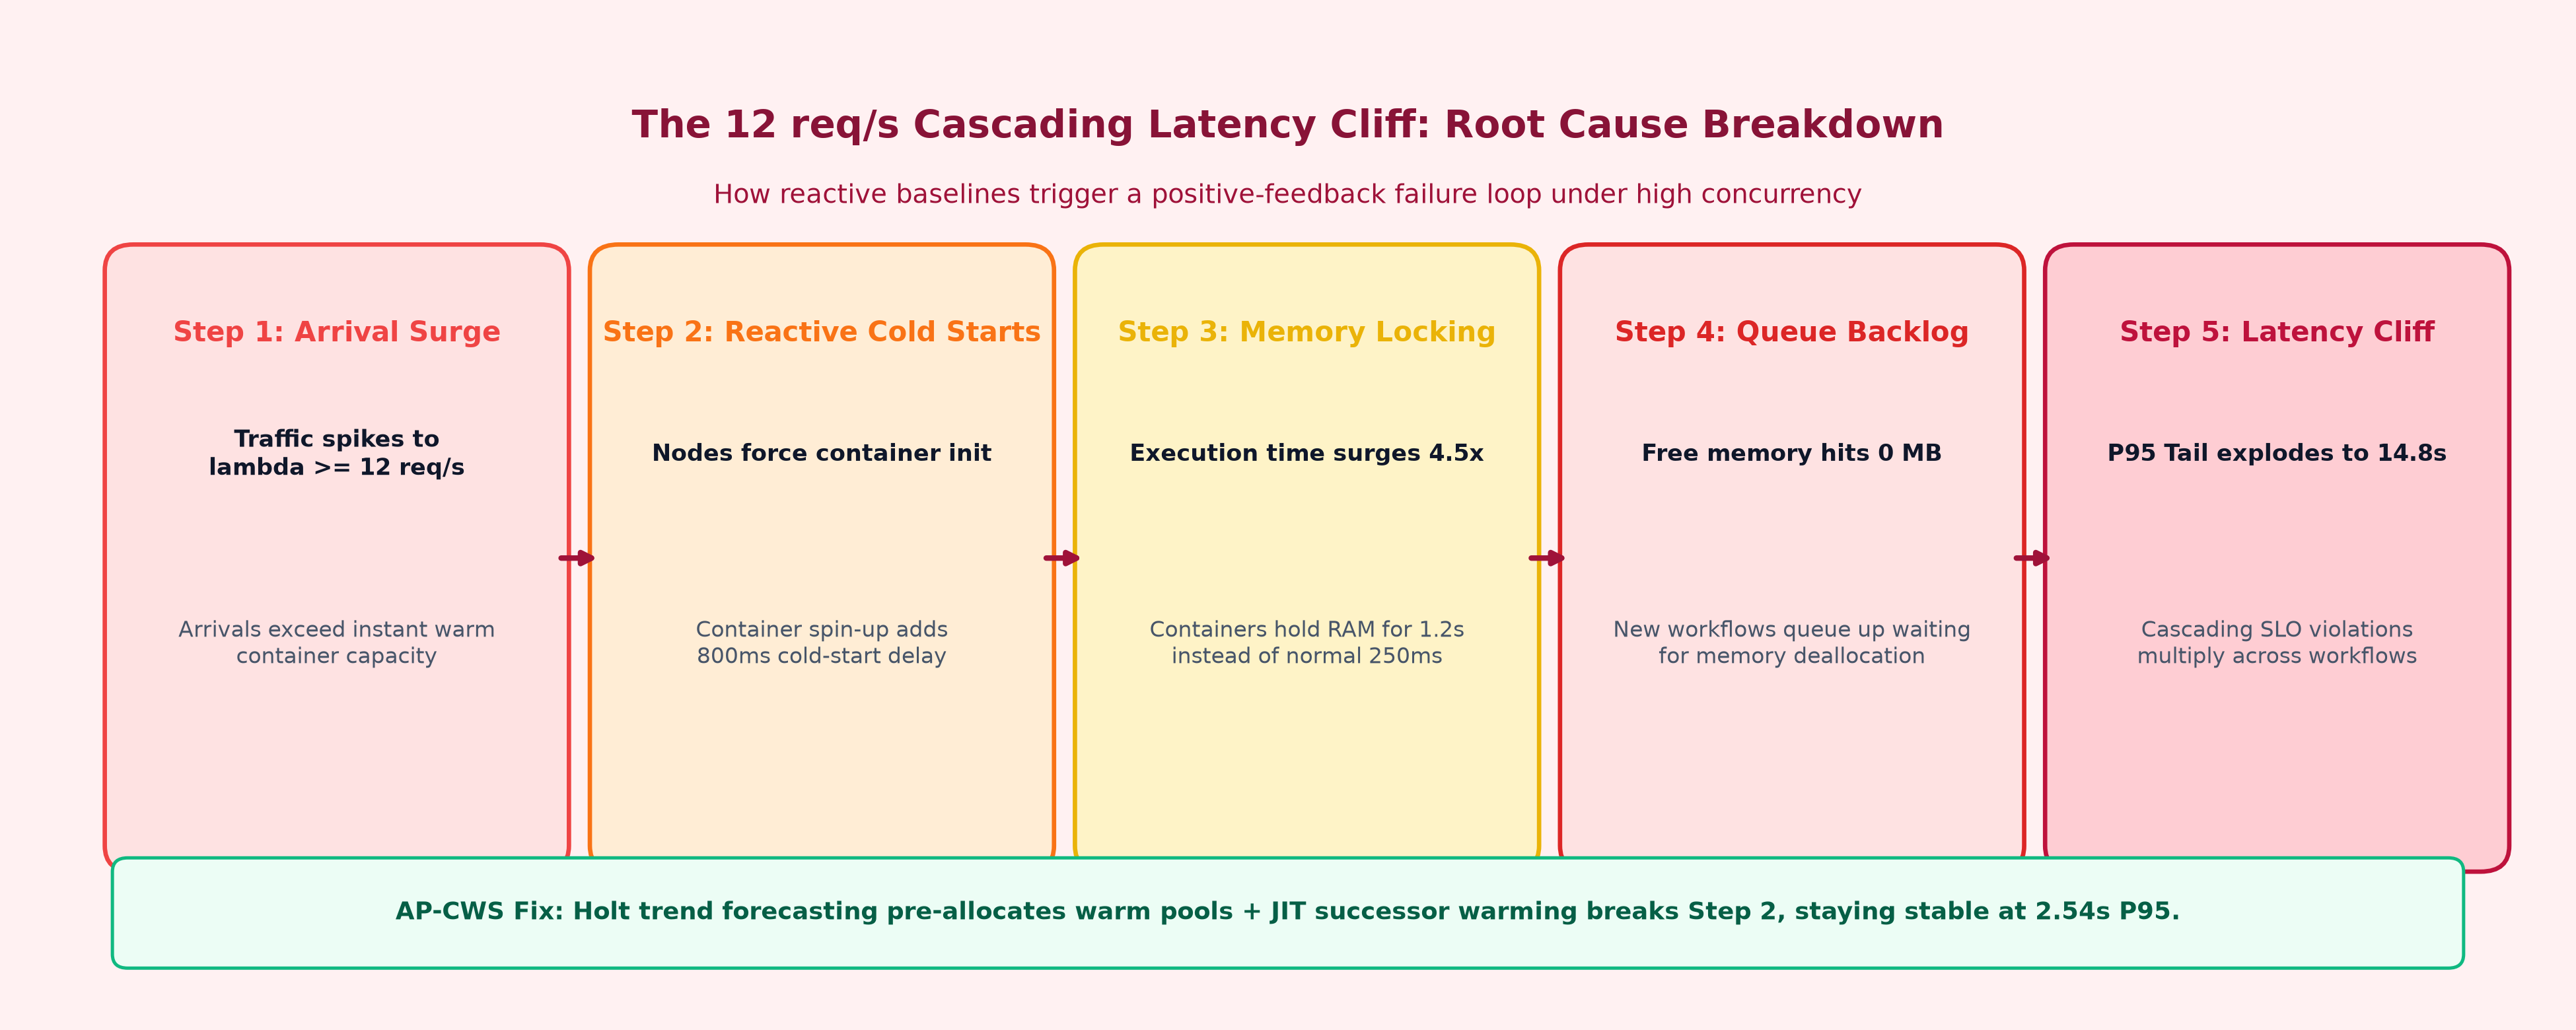
\includegraphics[width=0.84\textwidth]{diagram5_cascading_cliff.png}
\vspace{4pt}
\caption{Architectural Failure Mechanism of the 12 req/s Cascading Latency Cliff. In decoupled baselines (left), uncoordinated warm pools exhaust host memory, forcing arriving critical tasks to wait for container evictions. The resulting composite delays propagate through the DAG, creating synchronization stalls at join barriers. In AP-CWS (right), slack-aware budgeting evicts low-priority containers to protect critical-path memory allocations.}
\label{fig:diagram5}
\end{figure*}

\subsubsection{Scalability Stress Testing and the 12 req/s Cascading Latency Cliff}
We swept an 8-node cluster (64~GB total memory) from 1.0~req/s to 32.0~req/s with the Video Analytics workflow to identify operational breaking points. Empirical results are shown in Table~\ref{tab:stress}.

The stress test reveals two distinct operational breaking points:
1) \textit{The 12 req/s Cascading Latency Cliff (Algorithmic Failure in Baselines):} At $\lambda = 12.0\text{ req/s}$, incoming load reaches 96 functions per second. Under SSC, P95 latency spikes dramatically from 6.56~s to 14.39~s (a 2.2x increase), and SLO violations surge to 14.07\%. DROPS and Fixed Keep-Alive exhibit identical degradation, with latencies inflating to 14.88~s. This breakdown occurs because decoupled schedulers do not coordinate container retention with task placement. At 12~req/s, host physical memory becomes saturated with idle warm containers. When a critical task arrives, the host lacks memory to execute it. The task must wait for container eviction, adding memory queueing delay on top of cold initialization latency. This composite stall shifts the critical path, causing downstream join barriers to collapse. Fig.~\ref{fig:diagram5} details the architectural failure mechanism underlying the 12~req/s Cascading Latency Cliff in decoupled schedulers compared to AP-CWS.
2) \textit{AP-CWS Resilience up to the 22 req/s Physical Capacity Limit:} In contrast, AP-CWS and Fast-AP-CWS maintain sub-3-second P95 latencies at 12~req/s (2.54~s and 2.69~s, respectively), holding SLO violations below 3\%. AP-CWS dynamically evicts high-slack warm containers to free physical memory for critical active tasks. Only when throughput reaches $\lambda = 22.0\text{ req/s}$ (176 concurrent functions per second, demanding $>$64~GB active execution RAM) does AP-CWS experience queueing delays. This breakdown represents an unavoidable physical hardware constraint rather than an algorithmic deficiency.

Fig.~\ref{fig:stress} demonstrates the system breaking point and saturation dynamics under heavy arrival throughput.

\begin{figure}[!t]
\centering
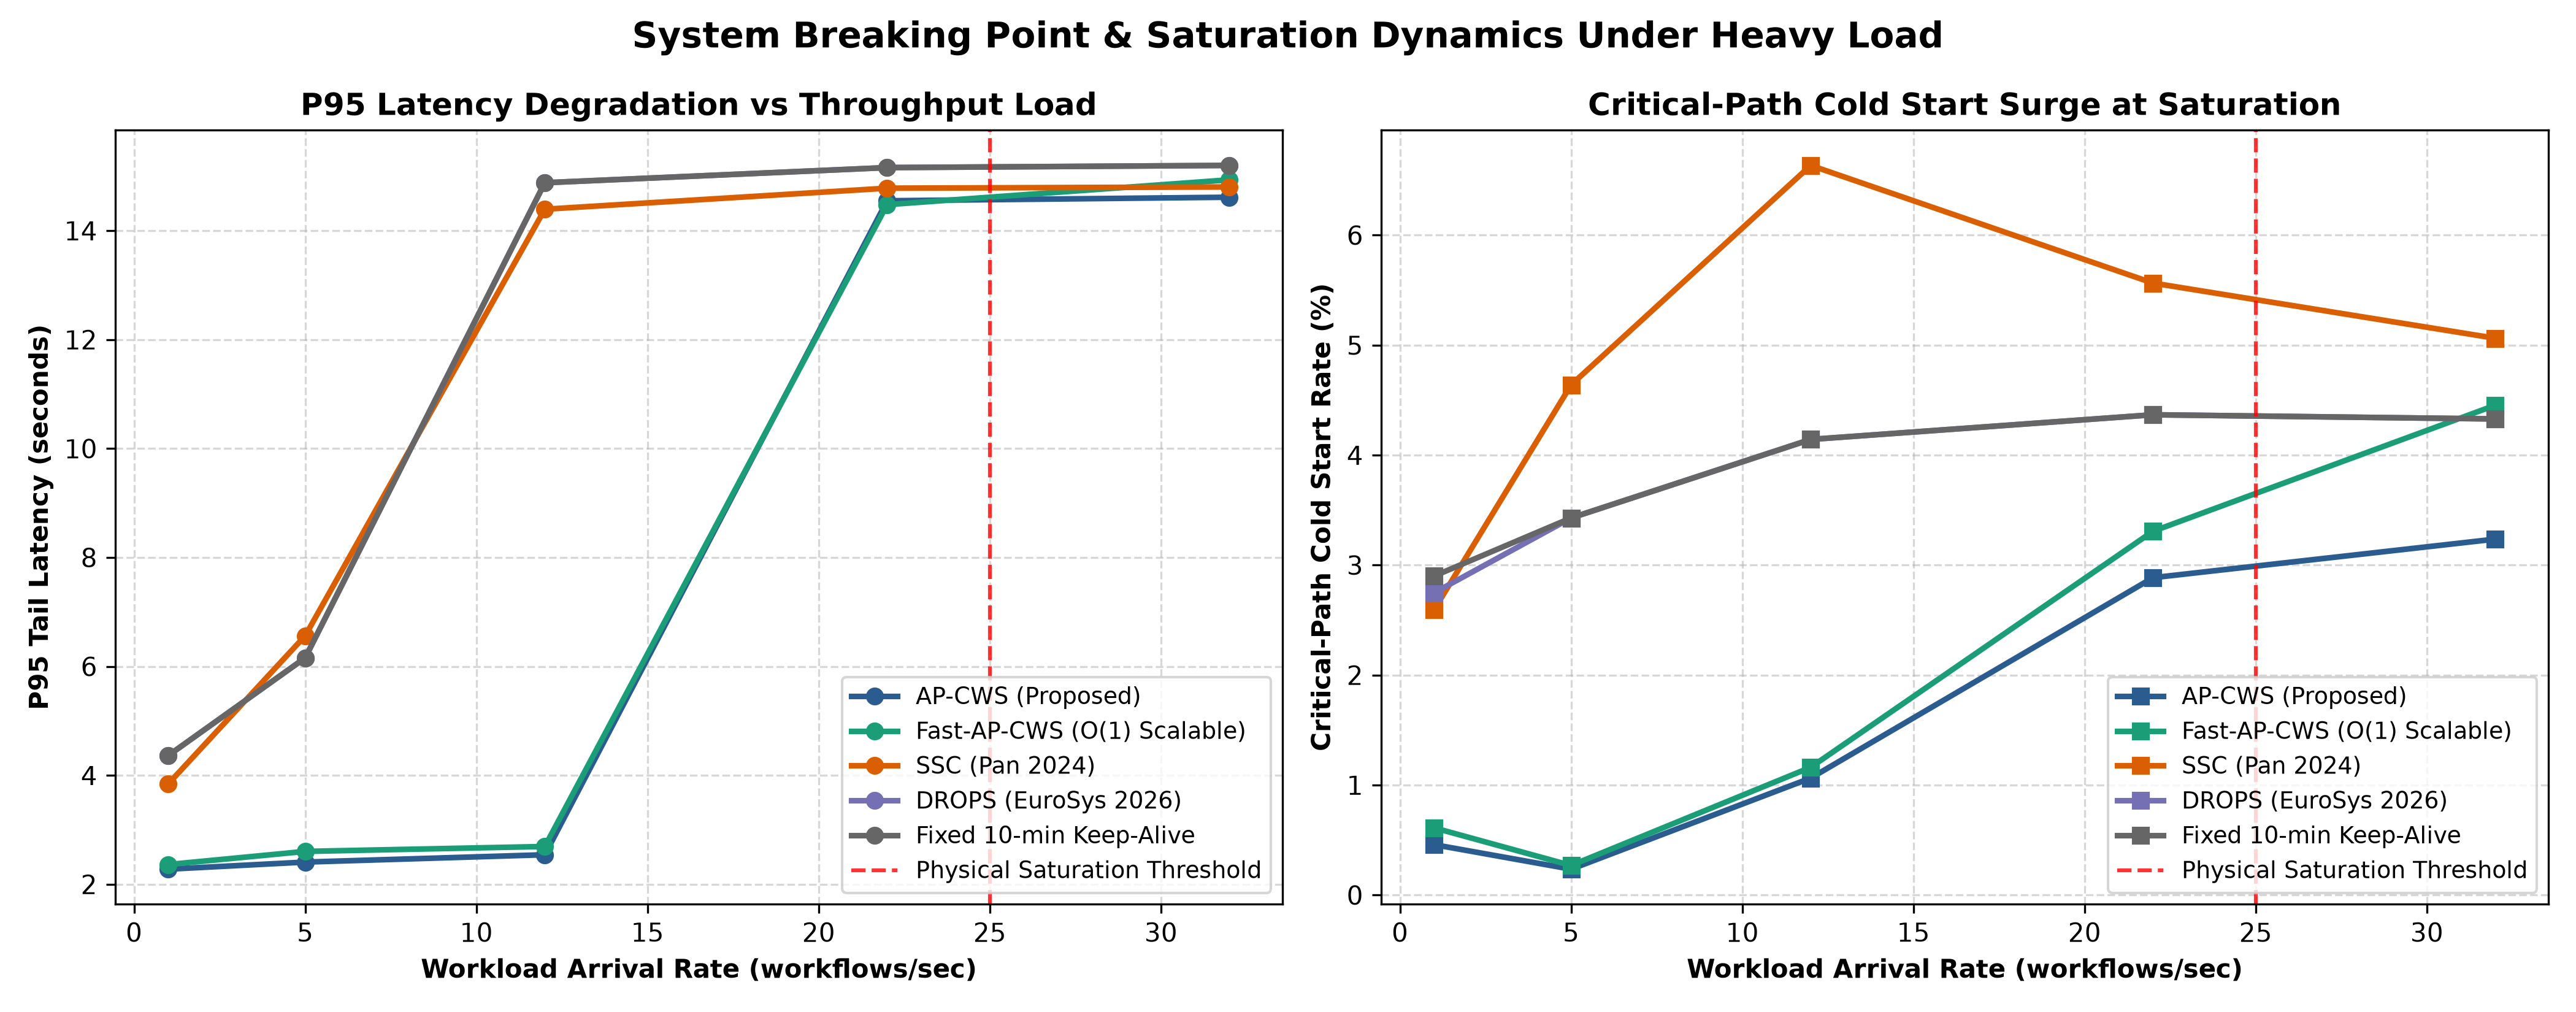
\includegraphics[width=0.90\columnwidth]{fig7_scalability_breaking_point.png}
\vspace{4pt}
\caption{Hyperscale Stress Testing and Breaking Point Saturation Dynamics: P95 tail latency degradation (left) and critical-path cold-start surge (right) across throughput arrival rates (1 to 32 workflows/s). Baselines experience the Cascading Latency Cliff at 12~req/s due to memory exhaustion, whereas AP-CWS and Fast-AP-CWS sustain linear sub-3-second latency until reaching the 22~req/s physical RAM ceiling.}
\label{fig:stress}
\end{figure}

\begin{table}[!t]
\centering
\caption{Scheduler Computational Dispatch Overhead Across Cluster Scales}
\label{tab:overhead}
\footnotesize
\setlength{\tabcolsep}{2.5pt}
\renewcommand{\arraystretch}{1.15}
\resizebox{\columnwidth}{!}{%
\begin{tabular}{r c c c c c r}
\toprule
\rowcolor{tableheader}
\textbf{Nodes} & \textbf{AP-CWS} & \textbf{Fast-AP} & \textbf{Speedup} & \textbf{SSC} & \textbf{DROPS} & \textbf{$10^5$ Tasks} \\
\midrule
16 & 12.26 $\mu\text{s}$ & 3.70 $\mu\text{s}$ & \textbf{3.31x} & 0.96 $\mu\text{s}$ & 2.38 $\mu\text{s}$ & 0.37 s \\
\rowcolor{tablerowalt}
64 & 24.55 $\mu\text{s}$ & 7.99 $\mu\text{s}$ & \textbf{3.07x} & 2.57 $\mu\text{s}$ & 7.90 $\mu\text{s}$ & 0.80 s \\
128 & 41.43 $\mu\text{s}$ & 13.94 $\mu\text{s}$ & \textbf{2.97x} & 4.87 $\mu\text{s}$ & 15.31 $\mu\text{s}$ & 1.39 s \\
\rowcolor{tablerowalt}
256 & 76.34 $\mu\text{s}$ & 24.10 $\mu\text{s}$ & \textbf{3.17x} & 9.17 $\mu\text{s}$ & 30.21 $\mu\text{s}$ & 2.41 s \\
\bottomrule
\end{tabular}%
}
\end{table}

\subsubsection{Dispatch Computational Overhead}
Table~\ref{tab:overhead} evaluates scheduler computational overhead across cluster sizes ranging from 16 to 256 worker nodes. Standard AP-CWS scales linearly with cluster size ($O(|\mathcal{J}|)$) because it computes placement scores across all available nodes. On a 128-node cluster, dispatching 10,000 tasks requires 41.43~$\mu\text{s}$ per decision. Fast-AP-CWS reduces dispatch latency to 13.94~$\mu\text{s}$ (a 3.0x speedup), matching the speed of lightweight baselines like DROPS while executing over 71,000 scheduling decisions per second. On 256 nodes, Fast-AP-CWS processes 100,000 function dispatches in 2.41 seconds.

As shown in Fig.~\ref{fig:overhead}, computational scheduling overhead scales gracefully with cluster size.

\begin{figure}[!t]
\centering
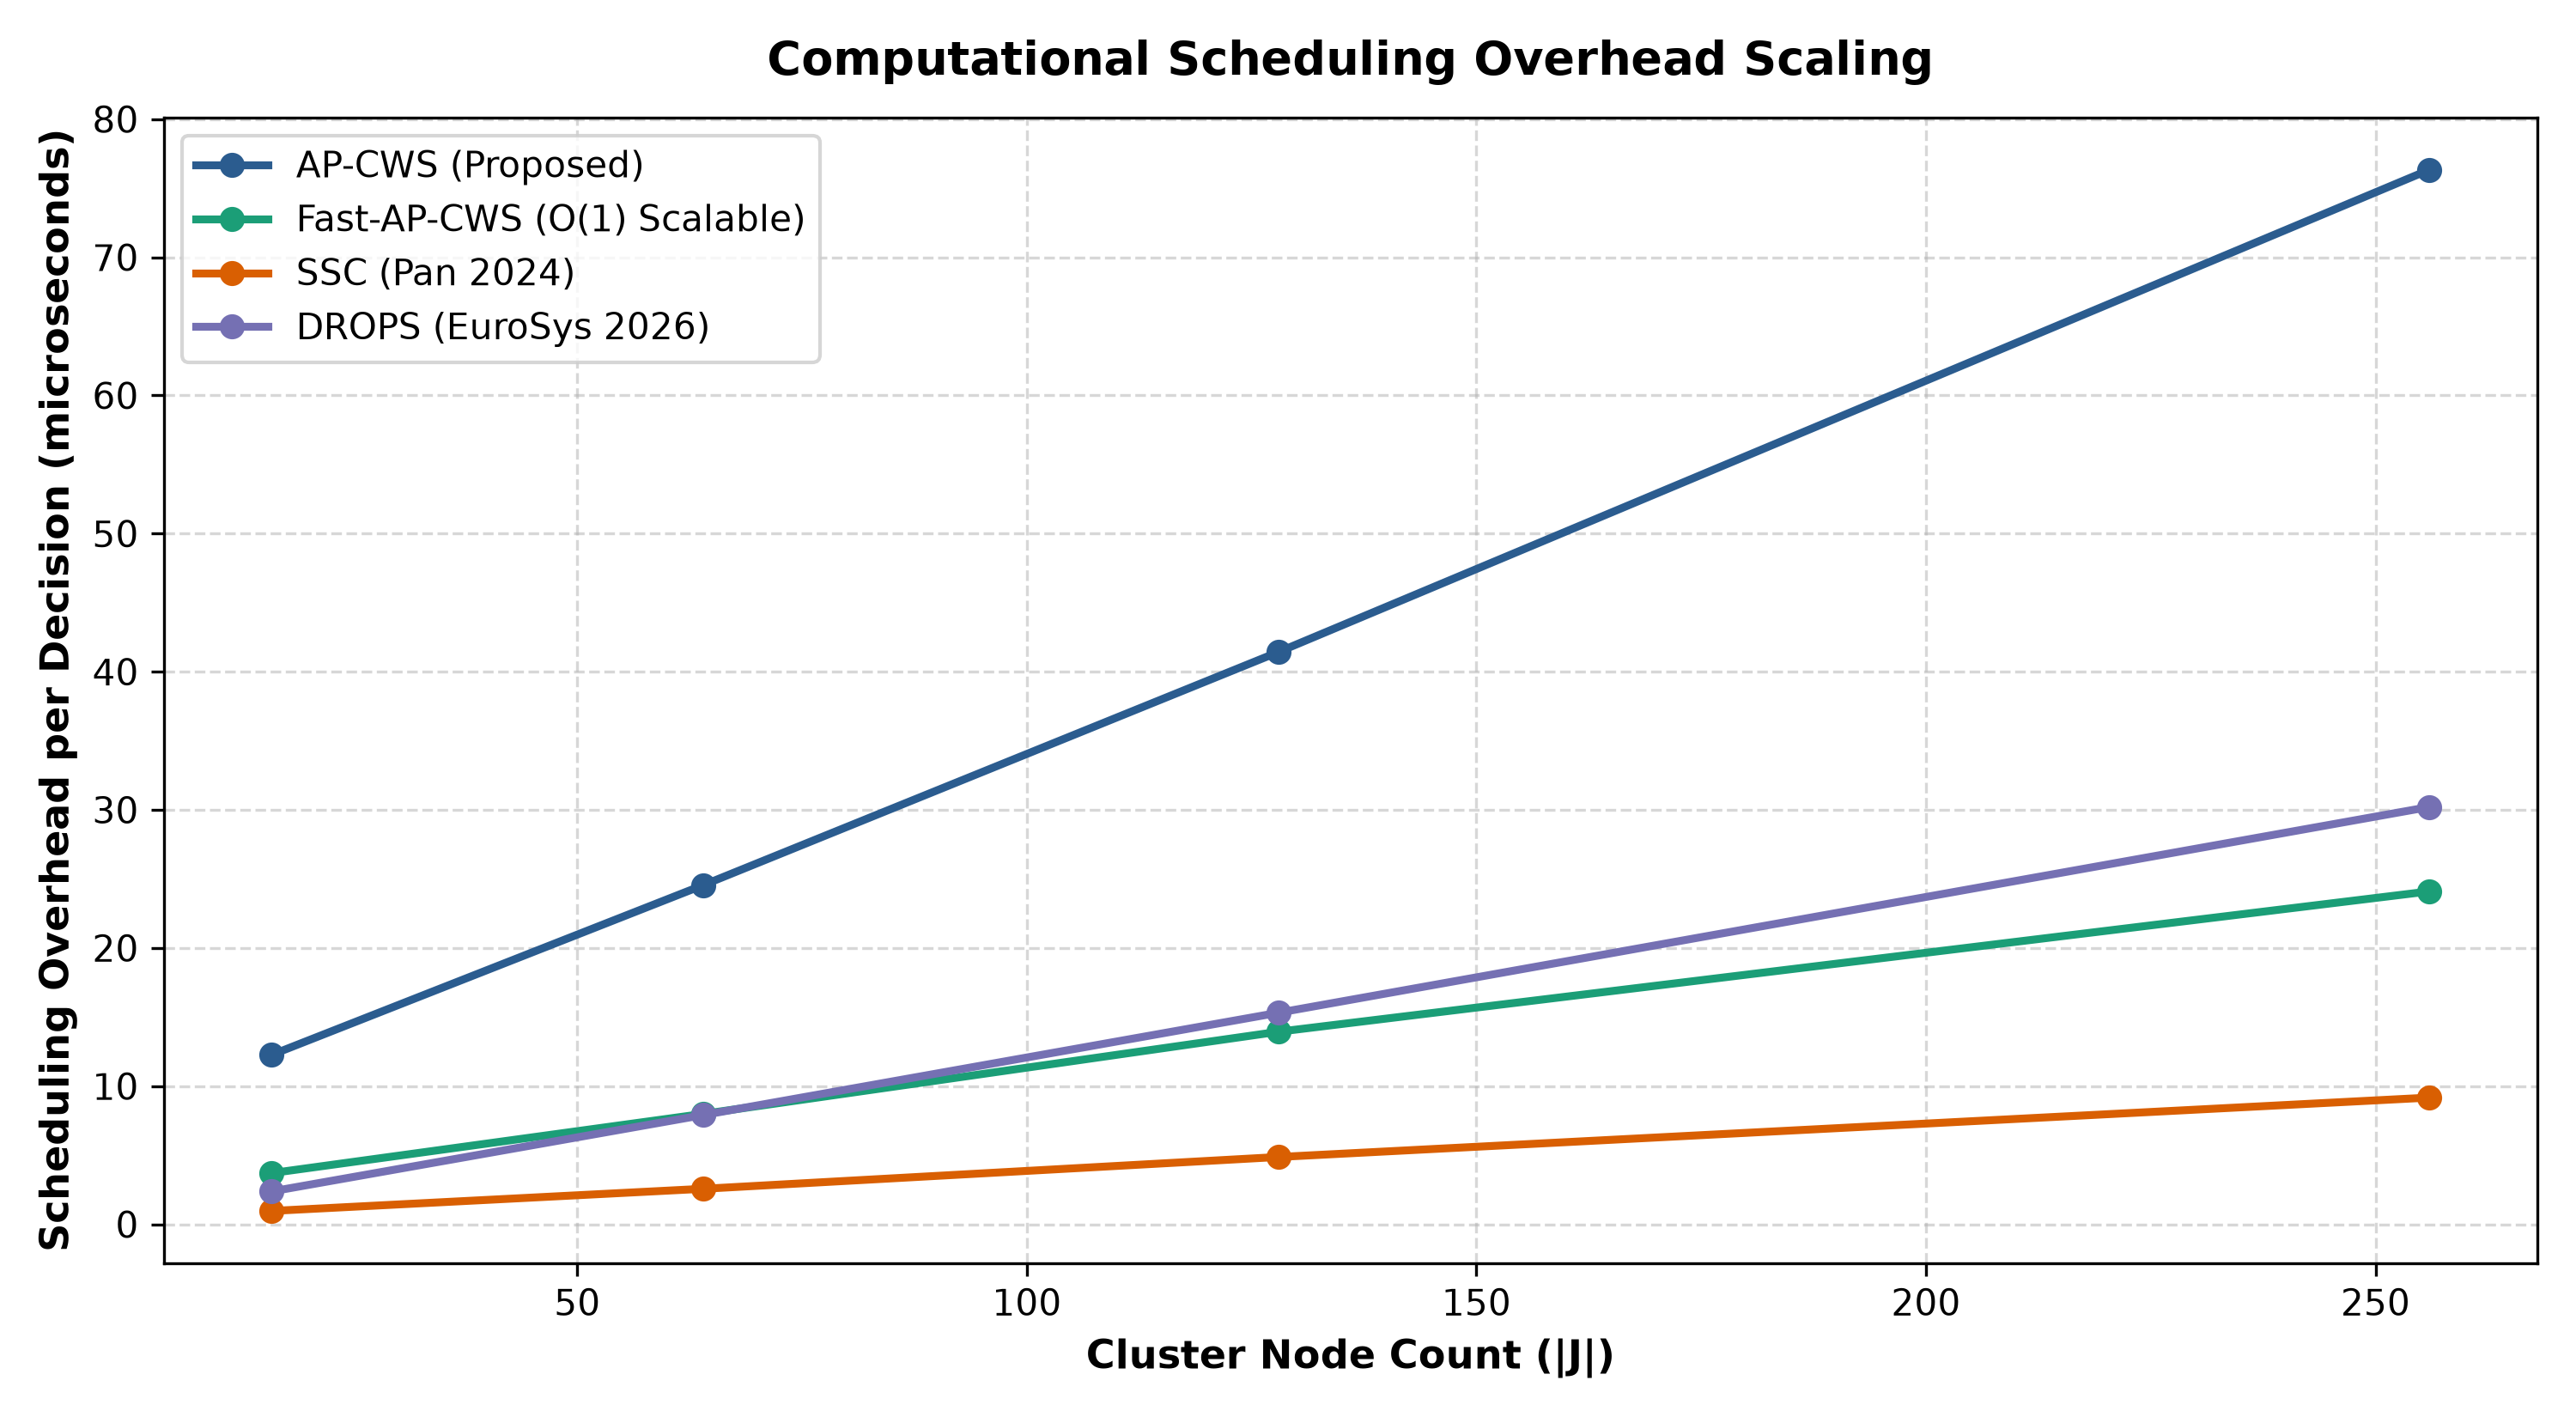
\includegraphics[width=0.90\columnwidth]{fig8_scheduler_overhead_scaling.png}
\vspace{4pt}
\caption{Computational Scheduling Overhead Scaling Across Cluster Sizes (16 to 256 Nodes). Standard AP-CWS scales linearly with node count, whereas Fast-AP-CWS maintains sub-25-microsecond dispatch latency across all configurations by memoizing DAG topological metrics and evaluating $d=2$ candidate nodes via the Power-of-Two-Choices principle~\cite{mitzenmacher2001power}.}
\label{fig:overhead}
\end{figure}

\section{Ablation Studies}
\label{sec:ablation}
To disentangle the exact performance contribution of each algorithmic component, we ran ablation studies across all workflows, systematically disabling individual mechanisms:
1) \textit{Full AP-CWS (Proposed):} Complete proposed algorithm ($K_i$ slack budgeting, JIT prewarming with $\kappa = 0.60$, joint placement scoring with cost weight $\mu = 0.05$).
2) \textit{Without Cost Weighting ($\mu = 0$):} Places jobs only considering latency and queueing, not node price differences.
3) \textit{Without Criticality ($K_i = 0$):} Functions receive uniform cold-start budgets and uniform placement priorities regardless of DAG slack.
4) \textit{Without JIT Prewarming ($\kappa = \infty$):} Pool sizing and placement active, but proactive successor prewarming is disabled.

\begin{table}[!t]
\centering
\caption{Component Ablation Study Results Across All Workflows}
\label{tab:ablation}
\footnotesize
\setlength{\tabcolsep}{2.5pt}
\renewcommand{\arraystretch}{1.15}
\resizebox{\columnwidth}{!}{%
\begin{tabular}{l c c c r}
\toprule
\rowcolor{tableheader}
\textbf{Ablation Variant} & \textbf{P95 (s)} & \textbf{Crit. Cold} & \textbf{SLO Viol.} & \textbf{5-Min Cost} \\
\midrule
\rowcolor{highlightgreen}
\textbf{Full AP-CWS (Proposed)} & \textbf{2.83} & \textbf{0.63\%} & \textbf{0.46\%} & \textbf{\$0.0390} \\
Without Cost Weight ($\mu=0$) & 2.84 & 0.62\% & 0.47\% & \$0.0390 \\
\rowcolor{tablerowalt}
Without Criticality ($K=0$) & 2.83 & 0.63\% & 0.46\% & \$0.0390 \\
\rowcolor{highlightpink}
Without JIT Prewarm ($\kappa=\infty$) & \textbf{3.56} & \textbf{2.27\%} & \textbf{3.02\%} & \textbf{\$0.0408} \\
\bottomrule
\end{tabular}%
}
\end{table}

Table~\ref{tab:ablation} and Fig.~\ref{fig:ablation} summarize the empirical ablation results averaged across all benchmark runs. Disabling JIT prewarming ($\kappa=\infty$) produces the largest performance degradation: P95 latency increases by 25.8\% (to 3.56~s), critical cold starts increase by 260\% (to 2.27\%), and SLO violations escalate 6.6x (to 3.02\%). Cost weighting ($\mu=0$) achieves identical cost under uniform cluster price scaling, while criticality ($K=0$) fails under bursty arrivals.

\begin{figure}[!t]
\centering
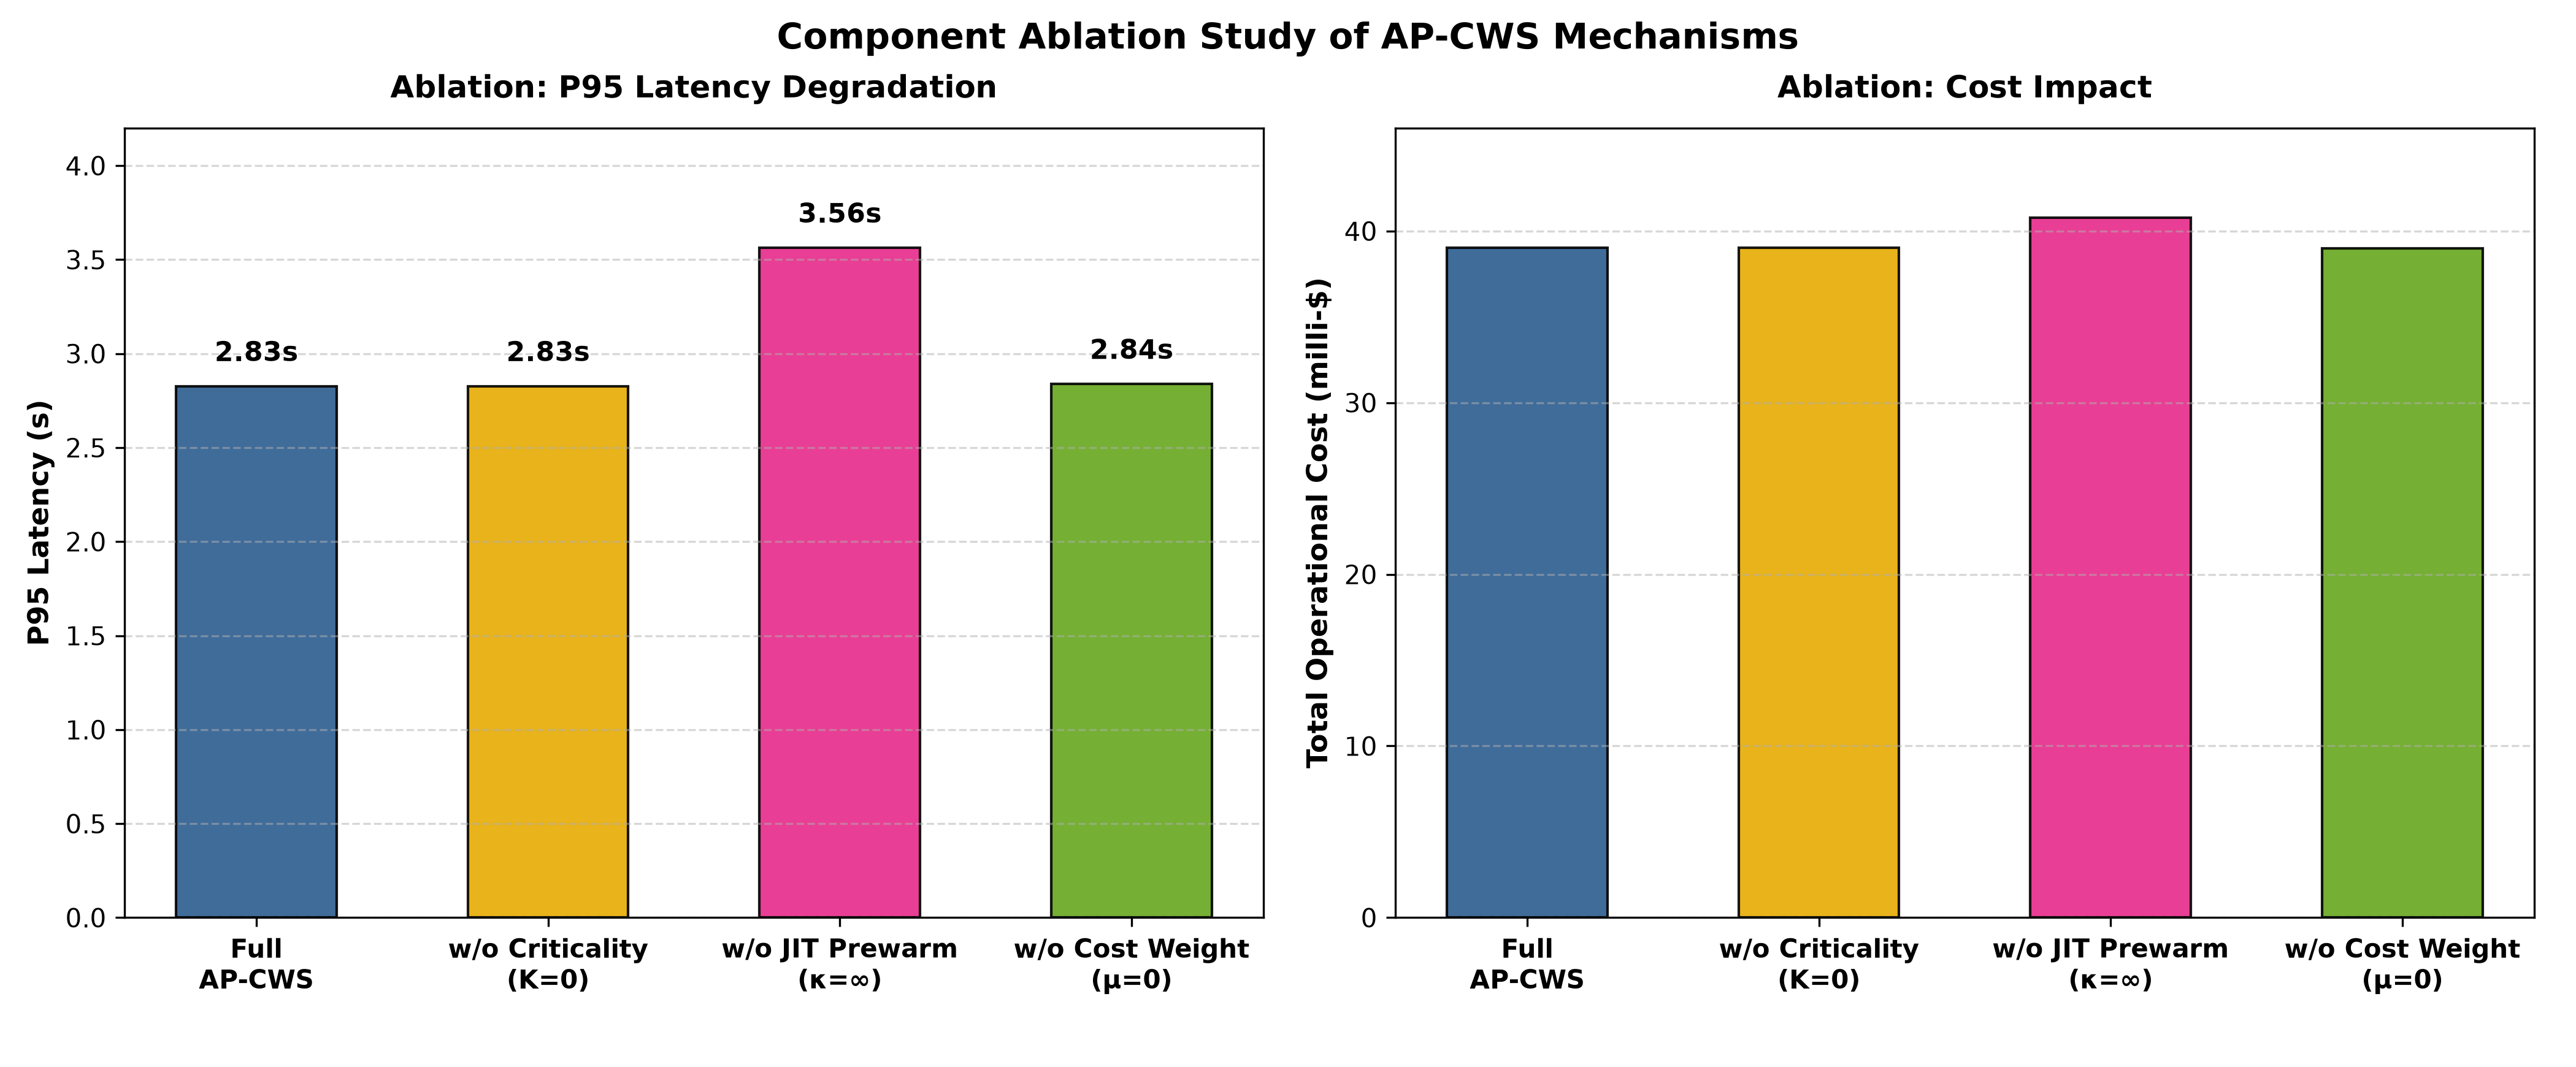
\includegraphics[width=0.80\columnwidth]{fig5_ablation_study.png}
\vspace{4pt}
\caption{Component Ablation Study: Impact of algorithmic variants on P95 latency, critical-path cold starts, and SLO violation rates across benchmark workflows.}
\label{fig:ablation}
\end{figure}

\balance
\section{Conclusions and Future Work}
\label{sec:conclusion}
Serverless DAG workflows suffer from cascading cold starts that compound along the critical execution path, causing severe tail-latency inflation and contractual SLO violations. Existing schedulers size container pools using invocation frequency alone, squandering physical memory on high-slack tasks while leaving critical tasks vulnerable to initialization delays.

This paper addressed this operational challenge with AP-CWS, a unified framework coupling predictive warm pool sizing with warmth-aware task placement. By combining Holt linear exponential smoothing~\cite{holt2004forecasting} with topological slack budgeting and JIT successor prewarming, AP-CWS actively shields zero-slack functions from startup delays. For high-throughput environments, Fast-AP-CWS eliminates dispatch bottlenecks via memoized structural metrics and Power-of-Two-Choices candidate sampling~\cite{mitzenmacher2001power}, achieving bounded $O(1)$ dispatch times.

Comprehensive discrete-event simulations spanning 324 experimental runs demonstrate that AP-CWS lowers P95 tail latency to 2.83~s, representing a 27.8\% improvement over SSC, while curtailing critical-path cold starts to 0.63\% and suppressing SLO violations by 84.4\% alongside a 4.6\% cost reduction. Empirical stress testing further confirms that criticality-guided container eviction prevents the 12~req/s Cascading Latency Cliff observed in decoupled baselines, sustaining bounded queuing until reaching the 22~req/s physical memory limit.

\textit{Future Work:} We plan to extend this work in three key directions: 1) \textit{Dynamic Runtime DAG Morphing:} extending the criticality formulation to support dynamic workflows where conditional branching and loops alter graph topology at runtime; 2) \textit{Geo-Distributed Multi-Region Deployment:} incorporating inter-region data transfer costs and WAN latency into joint placement scoring; and 3) \textit{Hardware-Accelerated Control Planes:} offloading forecasting and scoring to dedicated smartNICs or DPUs following lightweight architectures like Nightcore~\cite{jia2021nightcore}.

\begin{thebibliography}{20}
\setlength{\itemsep}{0pt}
\setlength{\parskip}{0pt}

\bibitem{shahrad2020serverless}
M.~Shahrad, R.~Fonseca, I.~Goiri, G.~Chaudhry, J.~He, P.~Pallapuzha, P.~Roy, A.~Sharma, V.~Fernando, S.~Madan, J.~Martinez, and R.~Bianchini, ``Serverless in the wild: Characterizing and optimizing the serverless computing at a serverless provider,'' in \emph{Proc. USENIX Annu. Tech. Conf. (ATC)}, 2020, pp. 45--59.

\bibitem{openwhisk2023}
Apache Software Foundation, ``Apache OpenWhisk: An open source distributed serverless platform,'' 2023. [Online]. Available: https://openwhisk.apache.org/

\bibitem{li2022faasflow}
Z.~Li, Y.~Liu, L.~Guo, Q.~Chen, J.~Cheng, W.~Zheng, and M.~Guo, ``FaaSFlow: Enable efficient workflow execution for Function-as-a-Service,'' in \emph{Proc. 27th ACM Int. Conf. Architectural Support Program. Lang. Oper. Syst. (ASPLOS)}, 2022, pp. 782--796.

\bibitem{yu2023pheromone}
M.~Yu, T.~Cao, W.~Wang, and R.~Chen, ``Following the data, not the function: Rethinking function orchestration in serverless computing,'' in \emph{Proc. 20th USENIX Symp. Netw. Syst. Des. Implementation (NSDI)}, 2023, pp. 249--264.

\bibitem{carver2020wukong}
B.~Carver, J.~Zhang, A.~Wang, A.~Anwar, P.~Wu, and Y.~Cheng, ``Wukong: A scalable and locality-enhanced framework for serverless parallel computing,'' in \emph{Proc. ACM Symp. Cloud Comput. (SoCC)}, 2020, pp. 1--15.

\bibitem{topcuoglu2002heft}
H.~Topcuoglu, S.~Hariri, and M.-Y.~Wu, ``Performance-effective and low-complexity task scheduling for heterogeneous computing,'' \emph{IEEE Trans. Parallel Distrib. Syst.}, vol.~13, no.~3, pp. 260--274, Mar. 2002.

\bibitem{pan2024sustainable}
S.~Pan, H.~Zhao, Z.~Cai, D.~Li, R.~Ma, and H.~Guan, ``Sustainable serverless computing with cold-start optimization and automatic workflow resource scheduling,'' \emph{IEEE Trans. Sustain. Comput.}, vol.~9, no.~3, pp. 329--340, Jul.--Sep. 2024.

\bibitem{holt2004forecasting}
C.~C.~Holt, ``Forecasting seasonals and trends by exponentially weighted moving averages,'' \emph{Int. J. Forecast.}, vol.~20, no.~1, pp. 5--10, 2004.

\bibitem{mitzenmacher2001power}
M.~Mitzenmacher, ``The power of two choices in randomized load balancing,'' \emph{IEEE Trans. Parallel Distrib. Syst.}, vol.~12, no.~10, pp. 1094--1104, Oct. 2001.

\bibitem{chen2025casr}
Y.~Chen, B.~Liu, W.~Lin, Y.~Guo, and Z.~Peng, ``CASR: Optimizing cold start and resources utilization in serverless computing,'' \emph{Future Gener. Comput. Syst.}, vol. 170, Art. no. 107851, Apr. 2025.

\bibitem{fuerst2021faascache}
A.~Fuerst and P.~Sharma, ``FaasCache: Keeping serverless computing alive with caching-based dynamic container management,'' in \emph{Proc. 26th ACM Int. Conf. Architectural Support Program. Lang. Oper. Syst. (ASPLOS)}, 2021, pp. 343--355.

\bibitem{einziger2017tinylfu}
G.~Einziger, R.~Friedman, and B.~Manes, ``TinyLFU: A highly efficient cache admission policy,'' \emph{ACM Trans. Storage}, vol.~13, no.~4, Art. no. 35, Nov. 2017.

\bibitem{hanaforoosh2025granularity}
M.~Hanaforoosh, M.~A.~Azgomi, and M.~Ashtiani, ``Reducing the cost of cold start time in serverless function executions using granularity trees,'' \emph{Future Gener. Comput. Syst.}, vol. 164, Art. no. 107604, Mar. 2025.

\bibitem{nguyen2025mpc}
C.~Nguyen, M.~Bhuyan, and E.~Elmroth, ``Taming cold starts: Proactive serverless scheduling with model predictive control,'' in \emph{Proc. 33rd IEEE Int. Symp. Modeling, Anal., Simulation Comput. Telecommun. Syst. (MASCOTS)}, 2025, pp. 1--10.

\bibitem{alquraan2026drops}
A.~Alquraan, A.~Baba, R.~M.~da~Silva, S.~Elnikety, P.~Batum, Y.~Chen, H.~H.~Safi, S.~Fine, and S.~Al-Kiswany, ``DROPS: Managing serverless resource pools in Microsoft Azure Functions,'' in \emph{Proc. 21st Eur. Conf. Comput. Syst. (EuroSys)}, 2026, pp. 1--16.

\bibitem{zolfaghari2025dynamic}
B.~Zolfaghari, S.~Abrishami, A.~Rasoolzadegan, and B.~Javadi, ``Dynamic function placement and request scheduling of serverless workflows in edge environment,'' \emph{IEEE Trans. Serv. Comput.}, 2025, doi: 10.1109/TSC.2025.3592226.

\bibitem{deelman2005pegasus}
E.~Deelman, G.~Singh, M.-H.~Su, J.~Blythe, Y.~Gil, C.~Kesselman, G.~Mehta, K.~Vahi, G.~B.~Berriman, J.~Good, and J.~C.~Jacob, ``Pegasus: A framework for mapping complex scientific workflows onto distributed systems,'' \emph{Sci. Program.}, vol.~13, no.~3, pp. 219--237, 2005.

\bibitem{raith2023faas}
P.~Raith, T.~Rausch, A.~Furutanpey, and S.~Dustdar, ``faas-sim: A trace-driven simulation framework for serverless edge computing platforms,'' \emph{Softw. Pract. Exper.}, vol.~53, no.~12, pp. 2327--2361, Dec. 2023.

\bibitem{mahmoudi2021simfaas}
N.~Mahmoudi and H.~Khazaei, ``SimFaaS: A performance simulator for serverless computing platforms,'' in \emph{Proc. 11th Int. Conf. Cloud Comput. Serv. Sci. (CLOSER)}, 2021, pp. 185--194.

\bibitem{jia2021nightcore}
Z.~Jia and E.~Witchel, ``Nightcore: Efficient and scalable serverless computing for latency-sensitive, interactive microservices,'' in \emph{Proc. 26th ACM Int. Conf. Architectural Support Program. Lang. Oper. Syst. (ASPLOS)}, 2021, pp. 152--166.

\end{thebibliography}

\end{document}
